\documentclass[aps,prd,reprint,nofootinbib,longbibliography]{revtex4-2}

\usepackage[T1]{fontenc}
\usepackage{amsmath,amsfonts,amssymb,bm}
\usepackage{graphicx}
\usepackage{booktabs}
\usepackage{xcolor}
\usepackage{braket}
\usepackage{mathtools}
\usepackage{multirow}
\usepackage{placeins}

\usepackage[
  colorlinks=true,
  linkcolor=blue,
  urlcolor=blue,
  citecolor=blue,
  anchorcolor=blue
]{hyperref}

% Figure 1 is drawn with TikZ-Feynman in the fonts of the paper when the package is installed;
% otherwise the prebuilt figures/fig0_diagrams.pdf (same source, scripts/make_diagrams.py) is used.
\IfFileExists{tikz-feynman.sty}{%
  \usepackage[compat=1.1.0]{tikz-feynman}%
  \tikzfeynmanset{warn luatex=false}%
  \newcommand{\diagramsfigure}{% Generated by scripts/make_diagrams.py; do not edit by hand.
{\small
\begin{tikzpicture}
  % (a) Type II tree diagram, t channel
  \begin{feynman}
    \vertex (g1) at (0.9, 2.2) {\(g(p_1)\)};
    \vertex (g2) at (0.9, 0.0) {\(g(p_2)\)};
    \vertex[crossed dot] (v1) at (3.2, 2.2) {};
    \vertex[crossed dot] (v2) at (3.2, 0.0) {};
    \vertex (a3) at (5.5, 2.2) {\(A(p_3)\)};
    \vertex (a4) at (5.5, 0.0) {\(A(p_4)\)};
    \diagram* {
      (g1) -- [gluon] (v1) -- [scalar] (a3),
      (g2) -- [gluon] (v2) -- [scalar] (a4),
      (v1) -- [gluon] (v2),
    };
  \end{feynman}
  \node[anchor=north west] at (-0.3, 2.75) {(a)};

  % (b) one-loop Type II diagram (crossed box); loop momentum k
  \begin{scope}[yshift=-3.7cm]
  \begin{feynman}
    \vertex (h1) at (0.9, 2.2) {\(g(p_1)\)};
    \vertex (h2) at (0.9, 0.0) {\(g(p_2)\)};
    \vertex (s1) at (2.0, 2.2);
    \vertex (s2) at (2.0, 0.0);
    \vertex[crossed dot] (e1) at (4.4, 2.2) {};
    \vertex[crossed dot] (e2) at (4.4, 0.0) {};
    \vertex (b1) at (5.7, 2.2) {\(A(p_3)\)};
    \vertex (b2) at (5.7, 0.0) {\(A(p_4)\)};
    \diagram* {
      (h1) -- [gluon] (s1) -- [gluon] (e1) -- [scalar] (b1),
      (h2) -- [gluon] (s2) -- [gluon] (e2) -- [scalar] (b2),
      (s1) -- [gluon] (e2),
      (s2) -- [gluon] (e1),
    };
    % momentum labels placed clear of the gluon coils
    \node at (3.2, 2.62) {\(k\)};
    \node at (3.2, -0.44) {\(p_4-p_1+k\)};
    \node[anchor=east] at (2.45, 1.55) {\(p_1-k\)};
    \node[anchor=west] at (3.95, 1.55) {\(p_3-k\)};
  \end{feynman}
  \node[anchor=north west] at (-0.3, 2.75) {(b)};
  \end{scope}
\end{tikzpicture}}
}%
}{%
  \newcommand{\diagramsfigure}{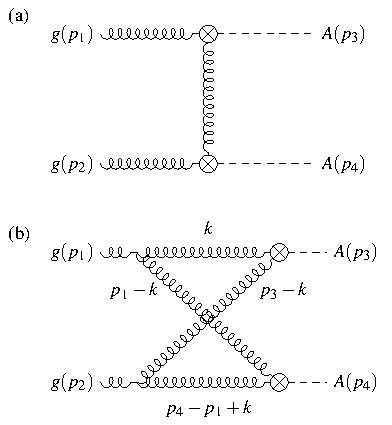
\includegraphics{figures/fig0_diagrams.pdf}}%
}

% Author metadata.
\newcommand{\PaperTitle}{Two-loop Type~II amplitudes for \texorpdfstring{$gg\to AA$}{gg to AA} near threshold and the double parton scattering singularity}
\newcommand{\PaperTitlePDF}{Two-loop Type II amplitudes for gg to AA near threshold and the double parton scattering singularity}
\newcommand{\PaperAuthor}{Arunima Bhattacharya}
\newcommand{\PaperAffiliation}{Theory Division, IFIC, University of Valencia-CSIC, E-46980 Paterna, Valencia, Spain}
\newcommand{\PaperEmail}{arunimab@ific.uv.es}

\newcommand{\as}{a_s}
\newcommand{\bA}{\beta_A}
\newcommand{\bH}{\beta_H}
\newcommand{\mA}{m_A}
\newcommand{\mH}{M_H}
\newcommand{\muR}{\mu_R}
\newcommand{\nf}{n_f}
\newcommand{\Nc}{N_c}
\newcommand{\Fin}{\mathrm{fin}}
\newcommand{\Ord}{\mathcal{O}}
\newcommand{\Li}{\operatorname{Li}}
\newcommand{\Real}{\operatorname{Re}}
\newcommand{\Imag}{\operatorname{Im}}
\newcommand{\dd}{\mathrm{d}}
\newcommand{\Mfull}[1]{\mathcal{M}^{(2),\Fin}_{#1}}
\newcommand{\Mflav}[2]{\mathcal{M}^{(2),\Fin}_{#1,#2}}
\newcommand{\abs}[1]{\left|#1\right|}
\providecommand{\lesssim}{\mathrel{\raisebox{-0.6ex}{$\stackrel{\textstyle<}{\sim}$}}}

% Generated by scripts/make_numbers.py from the data and results folders. Do not edit.
\newcommand{\AnglePointCount}{5}
\newcommand{\AngularReferenceChecks}{432}
\newcommand{\AngularSeriesChecks}{864}
\newcommand{\ArchiveOJShift}{0.03}
\newcommand{\ArchiveOneLoopDev}{\ensuremath{5\times10^{-56}}}
\newcommand{\ArchiveTwoLoopDev}{\ensuremath{5\times10^{-31}}}
\newcommand{\BasisCount}{8}
\newcommand{\BasisCountWord}{eight}
\newcommand{\BenchAlphaS}{0.118}
\newcommand{\BenchAs}{0.0094}
\newcommand{\BenchCos}{1/3}
\newcommand{\BenchCotBeta}{1}
\newcommand{\BenchMA}{125}
\newcommand{\BenchMt}{172.5}
\newcommand{\BenchMuR}{125}
\newcommand{\BenchNc}{3}
\newcommand{\BenchNf}{5}
\newcommand{\BetaPointCount}{9}
\newcommand{\BornSqrRatio}{1/4}
\newcommand{\BoseStatement}{are identical in all stored digits}
\newcommand{\CataniImagDigits}{15}
\newcommand{\ConstantCount}{13}
\newcommand{\ConstantCountWord}{thirteen}
\newcommand{\CrossoverBeta}{\ensuremath{1.7\times10^{-3}}}
\newcommand{\DPSBetaMax}{0.7}
\newcommand{\DPSBetaMin}{0.001}
\newcommand{\DPSMaxDeviation}{\ensuremath{3\times10^{-15}}}
\newcommand{\DPSNcValues}{3 and 4}
\newcommand{\DPSNfValues}{0, 2 and 5}
\newcommand{\EdgeBeta}{0.3}
\newcommand{\ExactComponentBeta}{1/10}
\newcommand{\ExactComponentCos}{1/3}
\newcommand{\ExactComponentCount}{six}
\newcommand{\ExactDigits}{160}
\newcommand{\ExactMaxComplete}{\ensuremath{1.3\times10^{-40}}}
\newcommand{\ExactMaxComponent}{\ensuremath{1.6\times10^{-40}}}
\newcommand{\ExactParameterSets}{three}
\newcommand{\ExactPointCount}{four}
\newcommand{\FeynmanDigits}{14}
\newcommand{\FileFactor}{64}
\newcommand{\FileFactorRoot}{8}
\newcommand{\ForwardBetaList}{$0.1$, $0.2$ and $0.3$}
\newcommand{\ForwardCosList}{$0.9$, $0.99$, $0.999$ and $-0.99$}
\newcommand{\ForwardCosMax}{0.999}
\newcommand{\ForwardSummary}{All values are below the maximum on the main grid at the same $\bA$, except for $\mathcal M_1$ at $\bA=0.1$, where the largest value, \ensuremath{1.23\times10^{-8}} at $c=0.999$, exceeds it by 21\%.}
\newcommand{\GJRatio}{-48}
\newcommand{\GridPointCount}{135}
\newcommand{\HHBetaMax}{0.7}
\newcommand{\HHBetaMin}{0.001}
\newcommand{\HHDpsMaxDev}{\ensuremath{3\times10^{-15}}}
\newcommand{\HHMtwoMax}{\ensuremath{3\times10^{-14}}}
\newcommand{\HHReproduceDigits}{40}
\newcommand{\ItwoNegativeFrom}{1/200}
\newcommand{\ItwoPositiveBetas}{$1/1000$ and $1/500$}
\newcommand{\LeadCheckedCount}{24}
\newcommand{\LeadOneOneNc}{1454+462\ln2+252\ln^22-42\pi^2+693\,i\pi-693L_\mu}
\newcommand{\LeadOneOneNf}{152+84\ln2+126\,i\pi-126L_\mu}
\newcommand{\LeadOneOnePrefactor}{\frac{\pi\Nc}{9}}
\newcommand{\LeadOneThree}{-\tfrac{28}{3}\pi\Nc^2}
\newcommand{\LeadOneTwo}{-\tfrac{14}{3}\pi\Nc(11\Nc-2\nf)}
\newcommand{\LeadPowerDevLarge}{0.3}
\newcommand{\LeadTwoOne}{-\tfrac{4}{3}\pi\Nc(4\Nc-\nf)}
\newcommand{\LeadTwoTwo}{-2\pi\Nc^2}
\newcommand{\LogRelationCubic}{- \tfrac{4 \Nc}{3}}
\newcommand{\LogShareBetaLarge}{0.1}
\newcommand{\LogShareBetaSmall}{0.01}
\newcommand{\LogShareLarge}{20}
\newcommand{\LogShareSmall}{30}
\newcommand{\LoopSizeBeta}{0.1}
\newcommand{\MoneOneLoopRatio}{1.1}
\newcommand{\MoneTwoLoopRatio}{0.7}
\newcommand{\MtwoOneLoopRatio}{2.3}
\newcommand{\MtwoRelation}{- 4 \Nc}
\newcommand{\OneLoopAgreementDigits}{30}
\newcommand{\OneLoopAone}{7\pi\Nc}
\newcommand{\OneLoopAzero}{-93.900+11.484\,i}
\newcommand{\OneLoopDigits}{400}
\newcommand{\OneLoopFitBetas}{$10^{-40}$ and $10^{-50}$}
\newcommand{\OneLoopMtwo}{\tfrac{1}{2}\pi\Nc}
\newcommand{\OneLoopScaleShift}{148.1}
\newcommand{\OneLoopScanNc}{3, 4 and 5}
\newcommand{\OneLoopScanNf}{0, 2 and 5}
\newcommand{\PSLQDigits}{110}
\newcommand{\PSLQResidual}{\ensuremath{4\times10^{-107}}}
\newcommand{\ParameterSetCount}{3}
\newcommand{\PhaseErrOnePointThree}{\ensuremath{5.94\times10^{-3}}}
\newcommand{\PhaseErrOnePointTwo}{\ensuremath{1.82\times10^{-4}}}
\newcommand{\PhaseErrTwoPointThree}{\ensuremath{6.04\times10^{-2}}}
\newcommand{\PhaseErrTwoPointTwo}{\ensuremath{1.89\times10^{-3}}}
\newcommand{\PhaseHigh}{-115.65}
\newcommand{\PhaseLow}{-141.65}
\newcommand{\PhaseSpread}{14.72}
\newcommand{\PhaseSpreadBeta}{3/10}
\newcommand{\PoneCancellationMax}{46.9\%}
\newcommand{\PoneCancellationMin}{42.2\%}
\newcommand{\PoneErrAtPointThree}{\ensuremath{1.10\times10^{-4}}}
\newcommand{\PoneErrLePointTwo}{\ensuremath{3.23\times10^{-6}}}
\newcommand{\PoneSlopeFour}{6.005}
\newcommand{\PoneSlopeSix}{8.005}
\newcommand{\PtwoErrAtPointThree}{\ensuremath{1.94\times10^{-3}}}
\newcommand{\PtwoErrLePointTwo}{\ensuremath{6.77\times10^{-5}}}
\newcommand{\PtwoSlopeFour}{5.955}
\newcommand{\PtwoSlopeSix}{8.034}
\newcommand{\PublishedTwoLoopMB}{204}
\newcommand{\QuadBetas}{$0.01$, $0.1$ and $0.3$}
\newcommand{\QuadNodes}{eight}
\newcommand{\QuadNodesRef}{32}
\newcommand{\QuadVoneDev}{\ensuremath{10^{-9}}}
\newcommand{\QuadVtwoDev}{\ensuremath{10^{-3}}}
\newcommand{\RGCoefficient}{3}
\newcommand{\RGCoefficientPublished}{192}
\newcommand{\RGSecondDev}{\ensuremath{1\times10^{-8}}}
\newcommand{\RGSets}{$(3,0,300\,\mathrm{GeV})$, $(3,5,125\,\mathrm{GeV})$ and $(4,2,150\,\mathrm{GeV})$}
\newcommand{\RGaDev}{\ensuremath{2\times10^{-7}}}
\newcommand{\RGbDev}{\ensuremath{2\times10^{-5}}}
\newcommand{\RatioBetaHigh}{3/10}
\newcommand{\RatioBetaLow}{1/10}
\newcommand{\RecommendedBeta}{0.2}
\newcommand{\RenormPointsWord}{seven}
\newcommand{\RhoHigh}{0.0628}
\newcommand{\RhoLow}{0.0401}
\newcommand{\ScalingFixedDev}{\ensuremath{6\times10^{-57}}}
\newcommand{\ScalingRawDev}{\ensuremath{7\times10^{-56}}}
\newcommand{\SeriesKB}{40}
\newcommand{\SigmaBeta}{0.1}
\newcommand{\SigmaLO}{\ensuremath{1.29\times10^{-8}}}
\newcommand{\SizeRatio}{5061}
\newcommand{\SqrtSPointThree}{262.1}
\newcommand{\SqrtSPointTwo}{255.2}
\newcommand{\SquareShareLarge}{4}
\newcommand{\SquareShareSmall}{21}
\newcommand{\ThresholdPercentPointThree}{4.83}
\newcommand{\ThresholdPercentPointTwo}{2.06}
\newcommand{\TimingBetas}{$1/10$, $1/5$ and $3/10$}
\newcommand{\TimingCos}{0}
\newcommand{\TimingExactMiB}{42.77}
\newcommand{\TimingFirstMax}{4.83}
\newcommand{\TimingFirstMedian}{3.92}
\newcommand{\TimingFirstMin}{3.84}
\newcommand{\TimingMA}{125}
\newcommand{\TimingMuR}{125}
\newcommand{\TimingNc}{3}
\newcommand{\TimingPrecision}{80}
\newcommand{\TimingRepeats}{seven}
\newcommand{\TimingRepresentationRatio}{70.4}
\newcommand{\TimingSeriesMiB}{0.61}
\newcommand{\TimingWarmMax}{19.22}
\newcommand{\TimingWarmMedian}{19.18}
\newcommand{\TimingWarmMin}{18.99}
\newcommand{\TopMassDPSA}{1.096}
\newcommand{\TopMassDPSB}{1.145}
\newcommand{\TopMassDPSC}{1.196}
\newcommand{\TopMassMAA}{125}
\newcommand{\TopMassMAB}{150}
\newcommand{\TopMassMAC}{170}
\newcommand{\TopMassPercentMax}{2.2}
\newcommand{\TopMassRatioA}{1.006}
\newcommand{\TopMassRatioB}{1.013}
\newcommand{\TopMassRatioC}{1.022}
\newcommand{\ValBetaMax}{3/10}
\newcommand{\ValBetaMin}{\ensuremath{10^{-3}}}
\newcommand{\ValCosMax}{2/3}
\newcommand{\ValidationRows}{1080}
\newcommand{\VirtualBetaMax}{0.3}
\newcommand{\VirtualBetaMin}{\ensuremath{10^{-3}}}
\newcommand{\VoneFit}{-1508.5}
\newcommand{\VoneFormulaDev}{\ensuremath{1\times10^{-10}}}
\newcommand{\VoneMax}{\ensuremath{1.08}}
\newcommand{\VoneMin}{\ensuremath{1.06}}
\newcommand{\VoneScaleDev}{\ensuremath{4\times10^{-12}}}
\newcommand{\VoneThreshold}{115.11}
\newcommand{\VtwoAngleSpread}{\ensuremath{5\times10^{-11}}}
\newcommand{\VtwoBetaLarge}{10^{-6}}
\newcommand{\VtwoBetaSmall}{10^{-8}}
\newcommand{\VtwoLogExact}{-155.446269}
\newcommand{\VtwoLogFit}{-155.446269}
\newcommand{\VtwoLogRelDiff}{\ensuremath{3\times10^{-11}}}
\newcommand{\VtwoLogScaled}{\ensuremath{-0.0137}}
\newcommand{\VtwoMax}{\ensuremath{1.03}}
\newcommand{\VtwoMin}{\ensuremath{0.79}}
\newcommand{\VtwoPeakBeta}{0.0041}
\newcommand{\VtwoPeakEll}{-4.85}
\newcommand{\VzeroBench}{8118}
\newcommand{\VzeroTwoMu}{15421}


\begin{document}

\title{Two-loop $gg\to AA$ amplitudes near threshold and the double parton scattering singularity}

\author{Arunima Bhattacharya\,
\href{https://orcid.org/0000-0003-4409-0901}
{
\includegraphics[scale=0.05]{orcidid.pdf}}}
\email{\PaperEmail}
\affiliation{Theory Division, IFIC, University of Valencia--CSIC,
E-46980 Paterna, Valencia, Spain}
%
%\title{\PaperTitle}
%\author{\PaperAuthor}
%\thanks{Contact author: \href{mailto:\PaperEmail}{\PaperEmail}}
%\affiliation{\PaperAffiliation}
%\date{\today}

\begin{abstract}
We study the two-loop Type II amplitudes for pseudoscalar pair production, $gg\to AA$, near threshold in the heavy top quark limit, where each pseudoscalar is emitted from its own effective gluon vertex. Their analytic forms contain large cancellations near threshold. We expand them in the pseudoscalar velocity $\beta_A$ through $\beta_A^6$ at fixed angle. After the endpoint constants are reduced, all inverse powers of $\beta_A$ and the odd powers through $\beta_A^5$ cancel, and every coefficient is even in $\cos\theta$. At leading power the angle enters only through the logarithm of the transverse momentum $p_T$. We identify the one-loop logarithm with the double parton scattering singularity: with the overall constant fixed at threshold, the factorised formula of Gaunt and Stirling reproduces the velocity dependence of its coefficient in the forward limit to $3\times10^{-15}$, and a one-loop $gg\to HH$ calculation confirms the CP-even weight with the same constant. At two loops, the equal-helicity amplitude grows as $\ln^3p_T$, and its logarithms follow the one-loop helicity weight in the forward limit at all velocities tested; the opposite-helicity amplitude, with no one-loop logarithm, grows as $\ln^2p_T$, and fits relate this term to the one-loop amplitude. In the finite virtual corrections, the one-loop logarithm does not interfere with the tree amplitude, and at two loops the highest logarithm, relative to the squared tree amplitude, is $-\tfrac{7}{64}\alpha_s^2N_c^2\ln^2(2p_T/m_A)$. The released remainders are normalised differently at different orders (a factor 64 at two loops, one-loop files at $\mu_R=1$ GeV); I convert them to a common normalisation, checked with the renormalisation group equations. For $0<\beta_A\leq0.2$, the series reproduce the complete remainders to $6.77\times10^{-5}$ at all tested points; they are released with an evaluator.
\end{abstract}

\maketitle

\section{Introduction}
\label{sec:introduction}

Neutral Higgs boson pairs of a two-Higgs-doublet model are produced at the LHC mainly by gluon fusion through top quark loops~\cite{Plehn:1996wb,Baglio:2023euv}. For pairs of pseudoscalars, $gg\to AA$, the next-to-leading order (NLO) QCD corrections were first computed in the limit of a heavy top quark~\cite{DawsonDittmaierSpira1998}, later matched to parton showers~\cite{Hespel:2014sla}, and recently obtained with the full dependence on the top quark mass~\cite{Baglio:2023euv}. In the benchmark point of Ref.~\cite{Baglio:2023euv} the full NLO cross section for $AA$ lies about $5\%$ below the Born-improved heavy top quark approximation at LHC energies, against about $12\%$ for $hH$, so the heavy top quark limit, with the exact mass dependence kept at leading order, is a reasonable starting point for higher orders. Beyond NLO only the two-loop virtual amplitudes in this limit are known~\cite{Bhattacharya:2019bmd}. For Standard Model Higgs pairs the corrections in the same limit are known to N$^3$LO~\cite{deFlorianMazzitelli2013NNLO,Banerjee:2018lfq,ChenEtAl2020}. Pairs of axion-like particles coupled to gluons are produced by the same mechanism, and non-resonant $gg\to aa$ production has recently been shown to constrain their interactions at the LHC~\cite{Brivio:2026alp}.

When the top quark is integrated out, the pseudoscalar couples to gluons through $G\tilde G$ and to light quarks through the divergence of the axial current. The amplitude for $gg\to AA$ then separates into two classes~\cite{Bhattacharya:2019bmd}. In Type~I both pseudoscalars originate from a single effective vertex. In Type~II each pseudoscalar is emitted from its own vertex and the two vertices are connected by gluon exchange in the $t$ or $u$ channel (Fig.~\ref{fig:diagrams}a). In the full theory the Type~II diagrams correspond to two top quark triangles joined by a gluon, the one-particle reducible contributions of Refs.~\cite{DawsonDittmaierSpira1998,Baglio:2023euv}; for Higgs pairs the corresponding class was computed at two loops in Ref.~\cite{Banerjee:2018lfq}. The two-loop Type~II finite remainders for $gg\to AA$ were obtained in closed form in Ref.~\cite{Bhattacharya:2019bmd}. They contain polylogarithms of weight up to four, among them $\Li_{2,2}$, and inverse powers of the Gram determinant $tu-\mA^4$, which vanishes at the pair threshold. The expressions occupy about \PublishedTwoLoopMB~MB, and large cancellations between their terms make them hard to evaluate close to threshold.

There are two reasons to study this region. The first is phenomenological. In the NLO predictions of Ref.~\cite{Baglio:2023euv} for $\mA=134.7$~GeV the invariant mass distribution of the pair is larger at $m_{AA}=300$~GeV, about 30~GeV above threshold, than at 400~GeV, and threshold resummation of this distribution requires at each $m_{AA}$ a hard function obtained from the infrared finite virtual amplitude~\cite{Sterman:1986aj,Catani:1989ne,deFlorian:2012za,deFlorian:2015moa,Bhattacharya:2021nsv}. The second concerns the analytic structure of loop amplitudes. When the transverse momentum $p_T$ of the final state particles vanishes, a one-loop amplitude with massless internal lines can have a Landau singularity~\cite{Landau:1959fi} in which each incoming parton splits into two collinear partons that then take part in two separate $2\to1$ scatterings. Gaunt and Stirling showed that this double parton scattering (DPS) singularity is at most logarithmic in $p_T$ for amplitudes of the Standard Model type, that for the processes they considered it requires the incoming partons to be in a state with $J_z=0$, and they gave a factorised formula for its coefficient~\cite{GauntStirling2011}. Dixon and Esterlis studied the corresponding singularity of six-gluon amplitudes in planar $\mathcal N=4$ super Yang--Mills theory to high loop order~\cite{DixonEsterlis2016}. As far as we are aware, it has not been examined beyond one loop in QCD at the level of amplitudes for a $2\to2$ process with a colour singlet final state; next-to-leading order corrections to the underlying splitting mechanism are known for double parton distributions~\cite{Diehl:2019rdh}. The Type~II amplitude has this topology: each incoming gluon can split into two gluons, which fuse pairwise into the two pseudoscalars at the effective vertices (Fig.~\ref{fig:diagrams}b). At threshold $p_T\to0$ at every scattering angle, so an expansion about threshold probes this region directly. In hadronic collisions the region in which both incoming partons split overlaps with double parton scattering in which both parton pairs arise from perturbative splittings, and the two contributions have to be combined without double counting~\cite{GauntStirling2011,DiehlGauntSchoenwald2017}; the related contribution with a splitting in one proton has been studied for pairs of Higgs bosons~\cite{GauntMaciulaSzczurek2014}.

In this paper we expand the two-loop Type~II finite remainders of Ref.~\cite{Bhattacharya:2019bmd} in the velocity $\bA$ of the pseudoscalars at fixed scattering angle, through $\bA^6$. Our main results are the following.
\begin{enumerate}
 \item After the endpoint constants of the expansion are expressed in a basis of \BasisCountWord{} constants, all inverse powers of $\bA$ and the odd powers through $\bA^5$ cancel, and every coefficient is even in $\cos\theta$, as required by Bose symmetry. At leading power the angle enters only through the logarithm of the transverse momentum of the pseudoscalars.
 \item This logarithm is the DPS singularity. At one loop its coefficient follows the factorised formula of Ref.~\cite{GauntStirling2011}, with the helicity weights of the splitting $g\to gg$ and the opposite signs of the amplitudes for $g^+g^+\to A$ and $g^-g^-\to A$. In the forward limit, where the momentum fractions depend on the velocity, and with the overall constant fixed at threshold, the formula reproduces the velocity dependence of the exact one-loop coefficient to \DPSMaxDeviation{} for $\DPSBetaMin\leq\bA\leq\DPSBetaMax$.
 \item At two loops the equal helicity amplitude grows as $\ln^3p_T$. The opposite helicity amplitude vanishes as $\bA^2$ at tree level and has no DPS logarithm at one loop, but grows as $\ln^2p_T$ at two loops. The ratio of the leading logarithms at two and one loops is the one found to all orders in planar $\mathcal N=4$ super Yang--Mills theory~\cite{DixonEsterlis2016}.
 \item In the finite virtual corrections to the cross section the one-loop logarithm cancels. At two loops $\ln^3p_T$ cancels, and the highest power is $\ln^2p_T$, with coefficient $-\tfrac74\pi^2\Nc^2$.
\end{enumerate}
We also find that the two-loop remainders released with Ref.~\cite{Bhattacharya:2019bmd} are larger by a factor of \FileFactor{} than the tree and one-loop amplitudes of the same reference, and that the released one-loop remainders omit their dependence on the renormalisation scale, so that they are correct only for $\muR=1$~GeV. We give all results in a consistent normalisation. The series reproduce the unexpanded remainders with relative errors of at most \PtwoErrLePointTwo{} for $\bA\leq\RecommendedBeta$; they are released together with an evaluator~\cite{SupplementalMaterial}.

The paper is organised as follows. Section~\ref{sec:setup} collects the conventions, the normalisation of the remainders and the counting of orders. Section~\ref{sec:expansion} describes the expansion and its accuracy. Section~\ref{sec:physics} discusses the leading power terms and their relation to the DPS singularity, and Sec.~\ref{sec:rate} their consequences for the cross section. We conclude in Sec.~\ref{sec:conclusions}.

\section{Amplitudes and conventions}
\label{sec:setup}


\subsection{Theoretical framework}

To study the threshold behaviour of $gg\to AA$ through two loops,
I use the amplitudes calculated in
Ref.~\cite{Bhattacharya:2019bmd} with the effective Lagrangian
of Eq.~\eqref{eq:EL}. The labels Type~I and Type~II follow
that reference and distinguish the two classes of diagrams.
They are unrelated to the Yukawa types of two-Higgs-doublet models.
The Type~II tree diagrams correspond, in the full theory, to
two top quark triangles connected by a gluon, i.e. the
one-particle reducible contribution of
Ref.~\cite{Baglio:2023euv}. Here I consider the contribution
with two $O_G$ insertions and omit the superscript
$\mathrm{II}$ from the amplitudes. Diagrams with one $O_G$
and one $O_J$ insertion first contribute at one loop.
Their coefficients are proportional to the $O_G$--$O_G$
tree coefficients, as discussed in
Sec.~\ref{sec:normalization}.

\begin{figure}[t]
 \centering
 \diagramsfigure
 \caption{(a) Type~II tree diagram in the $t$ channel; the $u$-channel diagram is obtained by exchanging the pseudoscalars. The crossed circles are the effective vertices of $O_G$. (b) One-loop Type~II diagram with loop momentum $k$. Its double parton scattering singularity lies at $k=xp_1$ and $p_3-k=(1-x)p_2$, where the four internal gluons are on shell and collinear with the incoming gluons: each incoming gluon splits into two, which fuse pairwise at the effective vertices. Gaunt and Stirling call this topology the crossed box~\cite{GauntStirling2011}.}
 \label{fig:diagrams}
\end{figure}



\subsection{Kinematics}

The Mandelstam variables are
\begin{align}
 \hat s&=(p_1+p_2)^2,
 &t&=(p_1-p_3)^2,
 &u&=(p_2-p_3)^2,
 \label{eq:mandelstam}
\end{align}
with $\hat s+t+u=2\mA^2$. Following the conventions of Ref.~\cite{Bhattacharya:2019bmd}, I use
\begin{align}
 \hat s&=\mA^2\frac{(1+x)^2}{x},
 &t&=-\mA^2 y,
 &u&=-\mA^2 z,
 \label{eq:xyz-definition}
\end{align}
with $x+x^{-1}=y+z$. With $c=\cos\theta$ in the partonic centre of mass frame,
\begin{align}
 \hat s&=\frac{4\mA^2}{1-\bA^2},
 &t,u&=\mA^2-\frac{\hat s}{2}(1\mp\bA c),
 \label{eq:stu-beta}
\end{align}
and the threshold substitution is
\begin{align}
 x&=\frac{1-\bA}{1+\bA},
 &y,z&=\frac{1+\bA^2\mp2\bA c}{1-\bA^2}.
 \label{eq:threshold-map}
\end{align}
All three variables tend to one as $\bA\to0^+$ at fixed $c$, and the expansion has to follow this correlated limit. The Gram determinant and the transverse momentum are
\begin{equation}
 tu-\mA^4
 =\frac{4\mA^4\bA^2(1-c^2)}{(1-\bA^2)^2},
 \qquad
 p_T^2=\frac{\mA^2\bA^2(1-c^2)}{1-\bA^2}.
 \label{eq:gram-scaling}
\end{equation}
Both vanish at threshold at every angle, and also at fixed $\bA$ when $c\to\pm1$.



\subsection{Tensor decomposition and helicity amplitudes}

With the overall factor $C_G^2$ removed, the amplitude is decomposed as
\begin{equation}
 \mathcal{M}^{\mu\nu}_{ab}
 =\delta_{ab}\left(T_1^{\mu\nu}\mathcal{M}_1+T_2^{\mu\nu}\mathcal{M}_2\right),
 \label{eq:tensor-decomposition}
\end{equation}
with
\begin{align}
 T_1^{\mu\nu}
 &=g^{\mu\nu}-\frac{p_1^\nu p_2^\mu}{p_1\!\cdot p_2},
 \label{eq:tensor-one}\\
 T_2^{\mu\nu}
 &=g^{\mu\nu}+\frac{1}{(p_1\!\cdot p_2)p_T^2}
 \Bigl[
 \mA^2p_2^\mu p_1^\nu
 -2(p_1\!\cdot p_3)p_2^\mu p_3^\nu
 \nonumber\\[-2pt]
 &\hspace{3.2em}
 -2(p_2\!\cdot p_3)p_3^\mu p_1^\nu
 +2(p_1\!\cdot p_2)p_3^\mu p_3^\nu
 \Bigr],
 \label{eq:tensor-two}\\
 p_T^2&=\frac{tu-\mA^4}{\hat s}.
 \label{eq:pt-definition}
\end{align}
For physical gluon polarisations, $T_1$ contributes only to equal helicities ($J_z=0$) and $T_2$ only to opposite helicities ($|J_z|=2$), each with a contraction of unit modulus. Up to phases the helicity amplitudes are~\cite{Glover:1987nx}
\begin{equation}
 \mathcal A_{\pm\pm}=C_G^2\,\mathcal M_1,
 \qquad
 \mathcal A_{\pm\mp}=C_G^2\,\mathcal M_2\,e^{\pm2i\phi},
 \label{eq:helicity}
\end{equation}
where $\phi$ is the azimuth of $\vec p_3$, and $\sum_{\mathrm{hel,col}}|\mathcal A|^2=2(\Nc^2-1)\,C_G^4\,(|\mathcal M_1|^2+|\mathcal M_2|^2)$. The labels 1 and 2 refer to the tensors, not to the diagram classes.

At tree level the two Type~II diagrams give
\begin{align}
 \mathcal M_1^{(0)}&=\frac{i\hat s}{2},
 \nonumber\\
 \mathcal M_2^{(0)}&=\frac{i\mA^2(x-z)(x^2+1)(xz-1)}{4xz(x^2-xz+1)}
 \nonumber\\
 &=2i\mA^2\bA^2(1-c^2)+\Ord(\bA^4),
 \label{eq:born}
\end{align}
in the variables of Eq.~\eqref{eq:xyz-definition}. I obtained Eq.~\eqref{eq:born} from the projections of the original calculation and checked it against a direct evaluation of the two Feynman diagrams with the vertex $iC_G\varepsilon_{\mu\alpha\rho\beta}k_1^\mu k_2^\rho\delta^{ab}$ that follows from Eq.~\eqref{eq:EL} (App.~\ref{app:normalization}). The suppression of $\mathcal M_2^{(0)}$ by $\bA^2$ is the centrifugal barrier of the $|J_z|=2$ state.


\subsection{Finite remainders and normalisation}
\label{sec:normalization}

The coefficients $\mathcal M_i$ of Eq.~\eqref{eq:helicity}, from which $C_G^2$ has been factored out, are expanded as
\begin{equation}
 \mathcal{M}_i
 =\mathcal{M}^{(0)}_i
 +\as\mathcal{M}^{(1)}_i
 +\as^2\mathcal{M}^{(2)}_i+\cdots,
 \label{eq:perturbative-expansion}
\end{equation}
with $\as$ renormalised at $\muR$.
The finite remainders, called the finite part in Ref.~\cite{Bhattacharya:2019bmd}, are defined by the IR subtraction of Refs.~\cite{Bhattacharya:2019bmd,Catani:1998bh},
\begin{align}
 \mathcal M^{(1)}&=2I^{(1)}\mathcal M^{(0)}+\mathcal M^{(1),\Fin},
 \nonumber\\
 \mathcal M^{(2)}&=4I^{(2)}\mathcal M^{(0)}+2I^{(1)}\mathcal M^{(1)}+\mathcal M^{(2),\Fin}.
 \label{eq:catani}
\end{align}
From here on $\mathcal M^{(n)}$ denotes the finite remainder
$\mathcal M^{(n),\Fin}$.

At two loops, I decompose each finite remainder into powers
of the number of light quark flavours,
\begin{equation}
 \Mfull{i}=\Mflav{i}{0}+\nf\,\Mflav{i}{1}+\nf^2\,\Mflav{i}{2}.
 \label{eq:nf-decomposition}
\end{equation}
Each $\Mflav{i}{k}$ is finite, but none is the amplitude of
a separate process: the term linear in $\nf$, for example,
combines the diagrams with a closed quark loop with the terms
of the renormalisation and of the infrared subtraction that
depend on $\nf$. In the rest of the paper, the complete
coefficient means $\Mfull{i}$ at $\nf=\BenchNf$.
Furthermore, the remainders released with Ref.~\cite{Bhattacharya:2019bmd} are normalised differently at different orders: the two-loop remainders carry an overall factor $\FileFactor$ relative to the tree and one-loop amplitudes, and the one-loop remainders are those for $\muR=1$~GeV. In the normalisation of Eq.~\eqref{eq:perturbative-expansion} the remainders are therefore
\begin{align}
 \mathcal M_i^{(1)}&=\mathcal M_{i,\mathrm{publ}}^{(1)}+2\beta_0\ln\frac{\muR^2}{\mathrm{GeV}^2}\,\mathcal M_i^{(0)},
 \nonumber\\
 \Mfull{i}&=\frac{1}{\FileFactor}\,\mathcal M_{i,\mathrm{publ}}^{(2)},
 \label{eq:normalisation}
\end{align}
with $\beta_0=(11\Nc-2\nf)/3$ and masses in GeV in the published expressions. The one-loop term restores the scale dependence required by renormalisation group invariance; with it, the released one and two-loop remainders are consistent with each other at every tested point. Appendix~\ref{app:normalization} gives the evidence. The logarithmic structure studied below, the expansion and its accuracy do not depend on these corrections; the one-loop constant and the finite virtual corrections of Sec.~\ref{sec:rate} do.

The one-loop amplitude with one $O_G$ and one $O_J$ insertion enters at $\Ord(\as^4)$, the order of the two-loop $O_G$--$O_G$ amplitude, since $C_J=\Ord(\as)\,C_G$. It is proportional to the tree amplitude: in the normalisation of Eqs.~(3.6) and (3.7) of Ref.~\cite{Bhattacharya:2019bmd},
\begin{equation}
 \mathcal M^{(1),\Fin}_{i,GJ,\mathrm{publ}}
 = \GJRatio\,\nf\,\mathcal M_i^{(0)},
 \qquad i=1,2,
 \label{eq:gj-proportional}
\end{equation}
at every point of the physical phase space. The proportionality is consistent with the axial anomaly, which relates the divergence of the flavour singlet axial current to the gluonic pseudoscalar operator~\cite{Adler:1969gk,Bell:1969ts,Larin1993}. At $\Ord(\as^4)$ the mixed contribution therefore has the kinematic dependence of the tree amplitude and adds no logarithm of $p_T$.

\subsection{Perturbative order}
\label{sec:counting}

The expansion in Eq.~\eqref{eq:perturbative-expansion} is
written for the coefficients $\mathcal M_i$, with the overall
factor $C_G^2$ removed.
The superscript $(n)$ counts loops of gluons and light quarks in the effective theory; in a two-Higgs-doublet model the top quark loops are contained in the Wilson coefficients.
The perturbative order of a contribution to the cross
section also depends on the powers of $\as$ in the Wilson
coefficients.

Since $C_G\propto\as$, the Type~II tree, one-loop and
two-loop contributions to the full amplitude are of
order $\as^2$, $\as^3$ and $\as^4$, respectively.
In a 2HDM, the leading amplitude is of Type~I and
starts at $\Ord(\as)$, giving a LO cross section
of order $\as^2$. Interference between the leading
Type~I amplitude and the Type~II tree amplitude
contributes at order $\as^3$, that is at NLO.
This is the one-particle reducible contribution to
the virtual corrections in
Refs.~\cite{DawsonDittmaierSpira1998,Baglio:2023euv}.
The Type~II two-loop amplitude first enters through
its interference with the leading Type~I amplitude
at order $\as^5$, or N$^3$LO. The same counting
applies to the corresponding class of amplitudes
for Higgs pairs~\cite{Banerjee:2018lfq}.

The mixed $O_G$--$O_J$ contribution discussed in
Sec.~\ref{sec:normalization} also contributes at
this N$^3$LO. In the heavy top quark theory,
$C_J=\Ord(\as)\,C_G$~\cite{Bhattacharya:2019bmd},
so its one-loop amplitude is of order $\as^4$,
the same as the two-loop $O_G$--$O_G$ amplitude.

When no Type~I amplitude is present, the Type~II
tree amplitude instead gives the LO cross section.
This is the case for an axion-like particle whose
only relevant interaction is its coupling to gluons
through $G\tilde G$. The one-loop and two-loop
terms in Eq.~\eqref{eq:perturbative-expansion}
then provide virtual contributions at NLO and
NNLO, respectively. The present results therefore
supply the $O_G$--$O_G$ part of the two-loop virtual
correction at NNLO for this process. A contact
interaction of dimension six containing two
pseudoscalars and two gluon fields would introduce
an additional Type~I amplitude, as in
Ref.~\cite{Brivio:2026alp}.


\subsection{Finite top quark mass effects}

The threshold expansion and the heavy top quark
approximation involve different limits. Taking
$\bA\to0$ places the pair invariant mass close to
$2\mA$, but imposes no restriction on $\mA/m_t$.
Finite top quark mass effects must therefore be
assessed separately when $A$ is the pseudoscalar of a 2HDM,
at values of $\tan\beta$ for which the top quark loop dominates.
No heavy top quark approximation is involved when
the coupling to $G\tilde G$ is specified directly
as an effective interaction, as in the axion-like
particle case above.

For the Type~II tree amplitude, the dependence on
the top quark mass is known. Each triangle in the
full theory couples a pseudoscalar to one on-shell
gluon and one virtual gluon. The two triangles in
a given channel have the same form factor, so the
contribution of each channel is multiplied, relative
to its heavy top quark limit, by
\begin{equation}
 \left[
 \frac{I_2(\tau_A,\lambda)}{I_2^\infty}
 \right]^2,
 \quad
 \tau_A=\frac{4m_t^2}{\mA^2},
 \quad
 \lambda=\frac{4m_t^2}{t}
 \quad\text{or}\quad
 \frac{4m_t^2}{u}.
 \label{eq:top-tree}
\end{equation}
Here $I_2$ is the loop function that also appears
in $A\to Z\gamma$, given in
Ref.~\cite{Baglio:2023euv}, and $I_2^\infty$
denotes its heavy top quark limit.
At the pair threshold, $t=u=-\mA^2$, so both channels have the same factor: \TopMassRatioA, \TopMassRatioB{} and \TopMassRatioC{} for $\mA=\TopMassMAA$, \TopMassMAB{} and \TopMassMAC~GeV, respectively, with $m_t=\BenchMt$~GeV. These differ from unity by at most about \TopMassPercentMax\%.

For the loop corrections, a partial estimate can
be made for the one-loop DPS logarithm. Its
coefficient involves the amplitudes for
$gg\to A$ with both gluons on shell, as discussed
in Sec.~\ref{sec:dps}. The relevant triangle form
factor is therefore obtained in the limit
$\lambda\to\infty$, rather than at the spacelike
virtuality of the exchanged gluon in the tree
diagrams:
\begin{equation}
 \frac{I_2(\tau_A,\infty)}{I_2^\infty}
 =\tau_A f(\tau_A),
 \qquad
 f(\tau)=\arcsin^2\!\left(\frac{1}{\sqrt{\tau}}\right).
 \label{eq:top-dps}
\end{equation}
If the DPS factorisation applies to the full
theory, with the top quark triangles treated as
hard subgraphs, the coefficient of the one-loop
logarithm is multiplied by $[\tau_A f(\tau_A)]^2$.
This gives \TopMassDPSA, \TopMassDPSB{} and
\TopMassDPSC{} for the same three masses, while
the velocity dependence and the helicity
selection rule would remain unchanged.
Neither this estimate nor the comparison of
tree amplitudes determines the finite top
quark mass corrections to the remaining
one-loop terms or to the complete two-loop
amplitude.

\section{Threshold expansion}
\label{sec:expansion}

\subsection{Construction}

After the substitution of Eq.~\eqref{eq:threshold-map}, each flavour coefficient is expanded at fixed $c$,
\begin{equation}
 \Mflav{i}{r}(\bA,c)
 =\sum_{n=-4}^{p}\sum_k
 C^{(i,r)}_{nk}\,\bA^n\ln^k\bA
 +\mathcal O_{\log}(\bA^{p+1}),
 \label{eq:series-structure}
\end{equation}
with $r=0,1,2$ and $p=4$ or 6. The coefficients $C^{(i,r)}_{nk}$ depend on $c$, $\mA^2$, $\muR^2$ and $\Nc$, and $\mathcal O_{\log}(\bA^n)$ stands for $\bA^n$ times a polynomial in $\ln\bA$. Inverse powers appear in intermediate steps because the tensor basis and the rational prefactors contain inverse Gram determinants, Eq.~\eqref{eq:gram-scaling}. They must be kept until all contributions at a given power have been combined.

The remainders contain logarithms, classical polylogarithms and the function $\Li_{2,2}$ of weight four~\cite{Frellesvig:2016ske,Vollinga:2004sn}, whose arguments approach correlated endpoints as $\bA\to0$. I expand the rational prefactors exactly and obtain the expansions of the special functions from differential equations in $\bA$, with boundary values at $\bA=0$. These equations have the iterated-integral form familiar from harmonic polylogarithms~\cite{RemiddiVermaseren2000} and from canonical differential equations for Feynman integrals~\cite{Henn2013}; the map $x=(1-\bA)/(1+\bA)$ is one of the transformations under which harmonic polylogarithms are closed~\cite{RemiddiVermaseren2000}. The method thus expands the known remainders, not the loop integrals, which could instead be expanded near threshold by the method of regions~\cite{BenekeSmirnov1998}. For the dilogarithm, for example, $\dd\Li_2(x)/\dd\bA=2(1-\bA^2)^{-1}\ln[2\bA/(1+\bA)]$ with $\Li_2(1)=\pi^2/6$ gives
\begin{align}
 \Li_2(x)
 &=
 \frac{\pi^2}{6}
 +2\bA\bigl[\ln(2\bA)-1\bigr]
 -\bA^2
 \nonumber\\
 &\quad
 +\bA^3
 \left[
   \frac{2}{3}\ln(2\bA)
   +\frac{1}{9}
 \right]
 -\frac{2}{3}\bA^4
 +\Ord\!\left(\bA^5\ln\bA\right).
 \label{eq:li2-threshold-example}
\end{align}
Since the prefactors start at $\bA^{-4}$, the special functions have to be expanded four orders beyond the final accuracy. The fourth and sixth order expansions were constructed independently, and all coefficients common to both agree.

\subsection{Endpoint constants and exact cancellations}
\label{sec:cancellations}
% Defined ahead of the citing text: a page-wide float can only appear at the top of a later page.
\begin{figure*}[t]
 \centering
 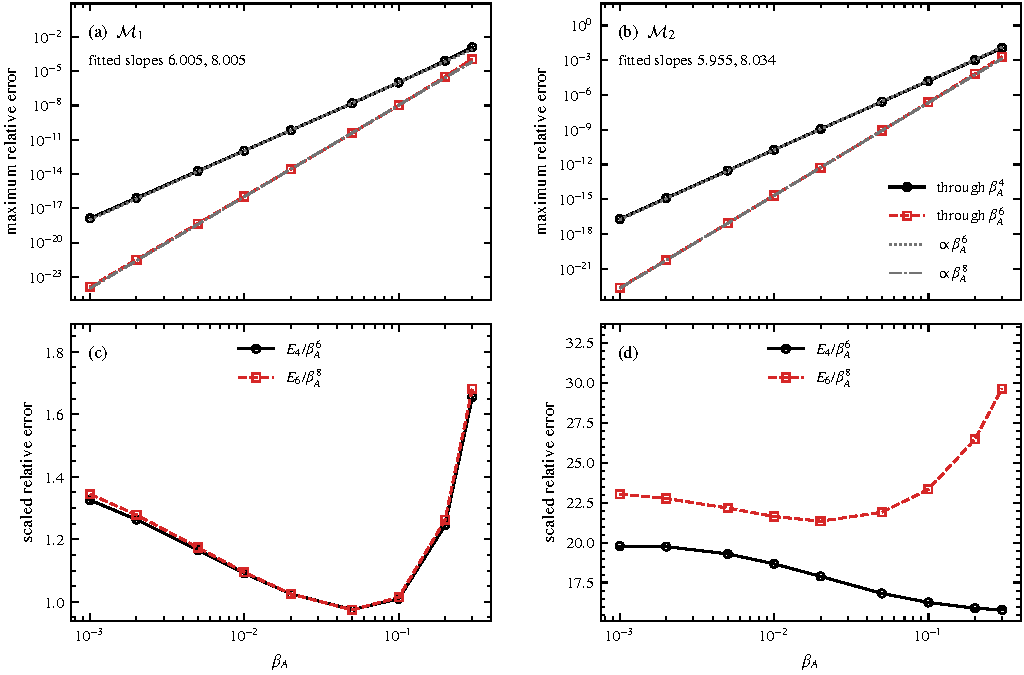
\includegraphics[width=0.98\textwidth]{figures/fig1_validation.pdf}
 \caption{Maximum relative errors of the complete two-loop coefficients after truncation at $\bA^4$ and $\bA^6$, with $\bA^6$ and $\bA^8$ for comparison (upper panels), and after division by these powers (lower panels). The maximum is taken over the five angles and three parameter sets of Table~\ref{tab:validation-grid}.}
 \label{fig:validation}
\end{figure*}


The boundary values at $\bA=0$ introduce \ConstantCountWord{} constants $\mathrm{MB}[p,q,a,w]$, defined in Eq.~\eqref{eq:mb-definition} of App.~\ref{app:constants}. Their arguments take the values $\pm1$ and $\tfrac12$, so they are alternating Euler sums of weight three and four~\cite{Blumlein:2009cf}. An integer relation search with the PSLQ algorithm~\cite{Ferguson:1999} at \PSLQDigits{} digits expresses each of them in the basis
\begin{equation}
 \{\zeta_3,\ \pi^2\ln2,\ \ln^32,\ \pi^4,\ \pi^2\ln^22,\ \ln^42,\ \Li_4(\tfrac12),\ \zeta_3\ln2\},
 \label{eq:constant-basis}
\end{equation}
with a largest residual of \PSLQResidual{} (Table~\ref{tab:mb-constants}).

With these reductions, and with the dilogarithms of $(1-c)/2$, $(c-1)/(c+1)$ and $(c+1)/(c-1)$ rewritten through $\Li_2\bigl((1+c)/2\bigr)$ by the reflection and Landen identities, every coefficient $C^{(i,r)}_{nk}$ becomes a polynomial in
\begin{equation}
 \bigl\{\ln\bA,\ \ln(1\pm c),\ \Li_2\bigl(\tfrac{1+c}{2}\bigr),\ \ln\tfrac{\mA^2}{\muR^2}\bigr\}\cup\{\ln2,\ \pi,\ \zeta_3,\ \Li_4(\tfrac12)\}
 \label{eq:function-basis}
\end{equation}
with coefficients rational in $c$ and $\Nc$. Treating these quantities as algebraically independent, I find that
\begin{enumerate}
 \item the coefficients of $\bA^{-4},\dots,\bA^{-1}$ vanish identically in every flavour coefficient;
 \item the coefficients of $\bA$, $\bA^3$ and $\bA^5$ vanish identically, so that through $\bA^6$ the expansion is a series in $\bA^2$ with logarithms;
 \item the coefficients of $\bA^0$, $\bA^2$, $\bA^4$ and $\bA^6$ of all six flavour coefficients, \LeadCheckedCount{} in total, are even in $c$, so that Bose symmetry holds order by order.
\end{enumerate}
The cancellations and the reductions of the constants were confirmed independently in Mathematica.

The cancellations have a simple origin. Exchanging the pseudoscalars exchanges $t$ and $u$, and the invariants that are symmetric under this exchange, $\hat s=4\mA^2/(1-\bA^2)$, $(t-u)^2=\hat s^2\bA^2c^2$ and $tu-\mA^4=\hat s\,p_T^2$ with $p_T^2=\hat s\bA^2(1-c^2)/4$, depend on $\bA$ only through $\bA^2$. No massive particle propagates in the loops, so the remainders are regular at $\hat s=4\mA^2$, and a colourless final state has no Coulomb singularity. Near threshold the only singularity is then the one at $p_T\to0$ discussed in Sec.~\ref{sec:dps}, which is logarithmic at one loop~\cite{GauntStirling2011}; the inverse Gram determinants of the tensor basis vanish at the same point but belong to the basis, not to the amplitude. A Bose symmetric function whose only singularity is logarithmic in $p_T^2$ is a series in $\bA^2$ with logarithms and has no inverse powers. At two loops this accounts for the cancellations found above but does not prove them, since there the logarithmic nature of the singularity is known only from the result itself. Table~\ref{tab:leading-threshold-inventory} lists the leading terms. Since the first omitted term is $\Ord_{\log}(\bA^{p+2})$, the truncation errors should scale as $\bA^6$ and $\bA^8$ for $p=4$ and 6.

\begin{table}[t]
\centering


\begin{tabular}{lccc}
\toprule
& inverse powers & leading & powers \\
quantity & in construction & power & of $\mathcal L$ \\
\midrule
$\Mflav{1}{0}$ & $\bA^{-2}$, $\bA^{-1}$ & $\bA^{0}$ & $0,1,2,3$ \\
$\Mflav{1}{1}$ & -- & $\bA^{0}$ & $0,1,2$ \\
$\Mflav{1}{2}$ & -- & $\bA^{0}$ & $0$ \\
$\Mflav{2}{0}$ & $\bA^{-4}$, $\bA^{-3}$, $\bA^{-2}$, $\bA^{-1}$ & $\bA^{0}$ & $0,1,2$ \\
$\Mflav{2}{1}$ & $\bA^{-1}$ & $\bA^{0}$ & $0,1$ \\
$\Mflav{2}{2}$ & -- & $\bA^{2}$ & $0$ \\
\bottomrule
\end{tabular}
\caption{Leading terms of the threshold expansion of the two-loop Type II remainders. The second column lists the inverse powers with nonzero coefficients in the construction files; they cancel identically after the reductions of Sec.~\ref{sec:cancellations}, as do all odd powers. The last column gives the powers of $\mathcal L$, Eq.~\eqref{eq:calL}, at leading power.}
\label{tab:leading-threshold-inventory}
\end{table}


The coefficient of $\nf^2$ is the simplest:
\begin{align}
 \Mflav{1}{2}(\bA,c)&=K+\Ord(\bA^2),
 \label{eq:nf2-leading-one}\\
 \Mflav{2}{2}(\bA,c)&=\bA^2(1-c^2)K+\Ord(\bA^4),
 \label{eq:nf2-leading-two}
\end{align}
where $K$ does not depend on the angle. It is the only flavour coefficient that follows the tree-level pattern $\mathcal M_2\propto\bA^2(1-c^2)$ of Eq.~\eqref{eq:born}, with the same ratio to the tree amplitude in both tensor structures. The complete expressions through $\bA^6$ are released as Wolfram Language files (App.~\ref{app:data}).

\subsection{Accuracy}
\label{sec:validation}

I compared the series with the unexpanded remainders at \BetaPointCount{} values of $\bA$ between \ValBetaMin{} and $\ValBetaMax$, \AnglePointCount{} angles and \ParameterSetCount{} choices of mass, scale and colour (Table~\ref{tab:validation-grid}). At each of the \GridPointCount{} points the test covers the six flavour coefficients and the two complete coefficients, \ValidationRows{} comparisons in total. Each unexpanded value is evaluated at increasing working precision until its real and imaginary parts are stable. The parameter set with $\Nc\neq3$ tests the colour dependence; all physical results use $\Nc=\BenchNc$. With the relative truncation error
\begin{equation}
 E_i^{(p)}
 =
 \frac{\left|\mathcal M_i^{[p]}-\mathcal M_i\right|}
      {\left|\mathcal M_i\right|},
 \qquad p=4,6,
 \label{eq:relative-error}
\end{equation}
where $\mathcal M_i$ is the unexpanded remainder and $\mathcal M_i^{[p]}$ its series through $\bA^p$. Fig.~\ref{fig:validation} shows the maximum over angles and parameter sets at each $\bA$. Fits give $E^{(4)}_i\propto\bA^{\PoneSlopeFour}$ and $\bA^{\PtwoSlopeFour}$, and $E^{(6)}_i\propto\bA^{\PoneSlopeSix}$ and $\bA^{\PtwoSlopeSix}$, as expected for a series in $\bA^2$. The lower panels divide out these powers. The ratios vary only slowly with $\bA$, because the first omitted coefficient contains powers of $\ln\bA$, and change most near $\bA=\EdgeBeta$, where the next order is no longer negligible; an error at a lower order would make them grow as an inverse power of $\bA$. For $\bA\leq\RecommendedBeta$ the sixth order series reproduces the complete coefficients with relative errors of at most \PoneErrLePointTwo{} and \PtwoErrLePointTwo; at $\bA=\EdgeBeta$ the errors are \PoneErrAtPointThree{} and \PtwoErrAtPointThree{} (Table~\ref{tab:AA-threshold-accuracy}). The values at $c$ and $-c$ \BoseStatement, in \AngularReferenceChecks{} comparisons of the unexpanded coefficients and \AngularSeriesChecks{} of the series.

\begin{table}[t]
\centering
\caption{Validation grid. At each point the six flavour coefficients and the two complete $\nf=\BenchNf$ coefficients are compared.}
\label{tab:validation-grid}
\begin{ruledtabular}
\begin{tabular}{ll}
quantity & values \\
\hline
$\bA$ & $1/1000$, $1/500$, $1/200$, \\
 & $1/100$, $1/50$, $1/20$, \\
 & $1/10$, $1/5$, $3/10$ \\
$c$ & $-2/3$, $-1/3$, $0$, $1/3$, $2/3$ \\
$(\mA/\mathrm{GeV},\,\muR/\mathrm{GeV},\,\Nc)$ & $(125,125,3)$, \\
 & $(125,250,3)$, \\
 & $(150,75,4)$ \\
\end{tabular}
\end{ruledtabular}
\end{table}


\begin{table}[!htb]
\centering
\caption{Maximum relative errors of the complete Type II coefficients on the validation grid. At each value of $\beta_A$, the maximum is taken over the \AnglePointCount{} angles and \ParameterSetCount{} parameter sets of Table~\ref{tab:validation-grid}.}
\label{tab:AA-threshold-accuracy}
\small
\setlength{\tabcolsep}{3pt}
\begin{ruledtabular}
\begin{tabular}{ccccc}
 & \multicolumn{2}{c}{$\mathcal{M}_1$ through} & \multicolumn{2}{c}{$\mathcal{M}_2$ through} \\
$\beta_A$ & $\beta_A^4$ & $\beta_A^6$ & $\beta_A^4$ & $\beta_A^6$ \\
\hline
0.01 & $1.09\times 10^{-12}$ & $1.09\times 10^{-16}$ & $1.87\times 10^{-11}$ & $2.16\times 10^{-15}$ \\
0.05 & $1.52\times 10^{-8}$ & $3.81\times 10^{-11}$ & $2.63\times 10^{-7}$ & $8.55\times 10^{-10}$ \\
0.10 & $1.01\times 10^{-6}$ & $1.01\times 10^{-8}$ & $1.63\times 10^{-5}$ & $2.33\times 10^{-7}$ \\
0.20 & $7.97\times 10^{-5}$ & $3.23\times 10^{-6}$ & $1.02\times 10^{-3}$ & $6.77\times 10^{-5}$ \\
0.30 & $1.21\times 10^{-3}$ & $1.10\times 10^{-4}$ & $1.15\times 10^{-2}$ & $1.94\times 10^{-3}$ \\
\end{tabular}
\end{ruledtabular}
\end{table}


The reference values were computed in Mathematica from the published expressions. I also evaluated these expressions with an independent code written in Python with mpmath~\cite{mpmath}, which has its own reader of the published files and computes $\Li_{2,2}$ from its defining double sum, with a one-dimensional integral representation where the sum converges slowly. At \ExactPointCount{} points covering the \ExactParameterSets{} parameter sets, the two complete coefficients agree with the reference values to a relative difference of at most \ExactMaxComplete, the precision to which the latter are stored; the \ExactComponentCount{} flavour coefficients at $\bA=\ExactComponentBeta$, $c=\ExactComponentCos$ agree to \ExactMaxComponent. The published expressions contain removable singularities at $c=0$, where $t=u$, which have to be taken as limits.

The expansion is carried out at fixed angle, but $p_T$ also vanishes when $c\to\pm1$ at fixed $\bA$. I therefore extended the comparison to $c=$ \ForwardCosList{} at $\bA=$ \ForwardBetaList{} (Table~\ref{tab:forward-angles}). \ForwardSummary{} The series thus remains accurate close to the beam, consistent with the absence of poles at $c=\pm1$ in its coefficients (Sec.~\ref{sec:leading}).

\begin{table}[t]
\centering
\caption{Relative truncation errors $E_i^{(6)}$ of the complete $\nf=\BenchNf$ coefficients towards the beam, at $\mA=\muR=\BenchMA\,\mathrm{GeV}$ and $\Nc=\BenchNc$. The last rows give the largest value on the grid of Table~\ref{tab:validation-grid}. The values at $c=-0.99$ equal those at $-c$.}
\label{tab:forward-angles}
\begin{ruledtabular}
\setlength{\tabcolsep}{3pt}
\begin{tabular}{llccc}
 & $c$ & $\bA=0.1$ & $\bA=0.2$ & $\bA=0.3$ \\
\hline
$\mathcal M_1$ & $0.9$ & $6.36\times10^{-9}$ & $1.11\times10^{-6}$ & $1.78\times10^{-5}$ \\
$\mathcal M_1$ & $0.99$ & $1.06\times10^{-8}$ & $2.43\times10^{-6}$ & $5.76\times10^{-5}$ \\
$\mathcal M_1$ & $0.999$ & $1.23\times10^{-8}$ & $2.96\times10^{-6}$ & $7.18\times10^{-5}$ \\
$\mathcal M_2$ & $0.9$ & $1.39\times10^{-7}$ & $3.08\times10^{-5}$ & $6.68\times10^{-4}$ \\
$\mathcal M_2$ & $0.99$ & $6.68\times10^{-8}$ & $1.47\times10^{-5}$ & $2.88\times10^{-4}$ \\
$\mathcal M_2$ & $0.999$ & $6.21\times10^{-8}$ & $1.65\times10^{-5}$ & $3.74\times10^{-4}$ \\
$\mathcal M_1$ & grid max. & $1.01\times10^{-8}$ & $3.23\times10^{-6}$ & $1.10\times10^{-4}$ \\
$\mathcal M_2$ & grid max. & $2.33\times10^{-7}$ & $6.77\times10^{-5}$ & $1.94\times10^{-3}$ \\
\end{tabular}
\end{ruledtabular}
\end{table}


\section{Leading power and the double parton scattering singularity}
\label{sec:physics}
% Defined ahead of the citing text: a page-wide float can only appear at the top of a later page.
\begin{table*}[!htb]
\centering
\caption{Coefficients of the leading power term, $\mathcal M_i|_{\beta_A^0}=m_A^2\sum_k \widehat A_{ik}\,\mathcal L^k$, with $\mathcal L$ of Eq.~\eqref{eq:calL}. They do not depend on the scattering angle. Exact forms for $\mu_R=m_A$ and general $N_c$, $n_f$; numerical values for $N_c=\BenchNc$, $n_f=\BenchNf$, $\mu_R=m_A$.}
\label{tab:leading-log-benchmark}
\begin{ruledtabular}
\begin{tabular}{cclrr}
 & $k$ & exact & $\operatorname{Re}\widehat A_{ik}$ & $\operatorname{Im}\widehat A_{ik}$ \\
\hline
$\mathcal M_1$ & $3$ & $-\tfrac{28}{3}\pi N_c^2$ & $-2.63894\times10^{2}$ & $0$ \\
$\mathcal M_1$ & $2$ & $-\tfrac{14}{3}\pi N_c(11N_c-2n_f)$ & $-1.01159\times10^{3}$ & $0$ \\
$\mathcal M_1$ & $1$ & Eq.~\eqref{eq:M1-L1} & $3.55129\times10^{3}$ & $4.76702\times10^{3}$ \\
$\mathcal M_1$ & $0$ & -- & $-3.98215\times10^{2}$ & $-4.00569\times10^{3}$ \\
$\mathcal M_2$ & $2$ & $-2\pi N_c^2$ & $-5.65487\times10^{1}$ & $0$ \\
$\mathcal M_2$ & $1$ & $-\tfrac{4}{3}\pi N_c(4N_c-n_f)$ & $-8.79646\times10^{1}$ & $0$ \\
$\mathcal M_2$ & $0$ & -- & $3.12007\times10^{2}$ & $3.40501\times10^{2}$ \\
\end{tabular}
\end{ruledtabular}
\end{table*}

% Defined ahead of the citing text: a page-wide float can only appear at the top of a later page.
\begin{figure*}[!ht]
 \centering
 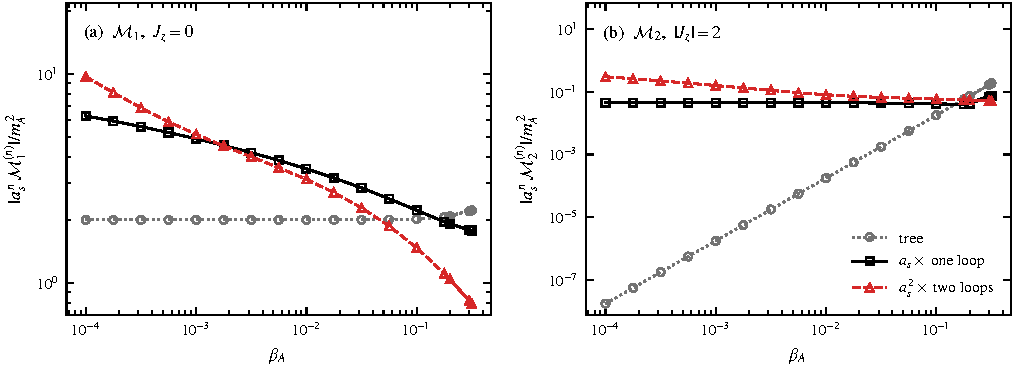
\includegraphics[width=0.94\textwidth]{figures/fig5_amplitudes.pdf}
 \caption{Tree-level, one-loop and two-loop terms of the Type~II amplitude, $|\as^n\mathcal M_i^{(n)}|/\mA^2$ with $\as=\BenchAs$ ($\alpha_s=\BenchAlphaS$), at $c=\BenchCos$, $\mA=\muR=\BenchMA\,\mathrm{GeV}$, $\Nc=\BenchNc$ and $\nf=\BenchNf$. Tree level: Eq.~\eqref{eq:born}; one loop: remainder of Ref.~\cite{Bhattacharya:2019bmd} with the scale dependence of Eq.~\eqref{eq:normalisation} restored; two loops: series through $\bA^6$. $\mathcal M_1$ and $\mathcal M_2$ are the equal and opposite helicity amplitudes, Eq.~\eqref{eq:helicity}.}
 \label{fig:amplitudes}
\end{figure*}


\subsection{Leading power}
\label{sec:leading}

To determine the leading threshold behaviour of the
two-loop remainders, I first collect the terms of
order $\bA^0$, including all powers of $\ln\bA$
that multiply them. The notation $\big|_{\bA^0}$ used below
denotes this part of the expansion.

In the expanded remainders, the logarithms of $\bA$ and of the angular
variables appear at leading power in the combination
$\ln\bA+\tfrac12\ln(1-c^2)$. I therefore introduce
\begin{align}
 \mathcal L
 &=\ln\bA+\tfrac12\ln(1-c^2)+\ln2+\frac{i\pi}{2}
 \nonumber\\
 &=\tfrac12\ln\bigl[-4\bA^2(1-c^2)\bigr],
 \label{eq:calL}
\end{align}
where the logarithm of the negative argument is taken on the branch
$\ln(-X)=\ln X+i\pi$ for $X>0$, which is the one followed by the remainders
in the physical region.

The meaning of $\mathcal L$ follows from Eq.~\eqref{eq:gram-scaling}.
Substituting the expressions for $tu-\mA^4$ and $p_T^2$ gives
\begin{align}
 \nonumber
 \mathcal L
 &=\tfrac12\ln\frac{\mA^4-tu}{\mA^4}
   +\ln(1-\bA^2)
 \\
 &=\ln\frac{2p_T}{\mA}+\frac{i\pi}{2}
   +\tfrac12\ln(1-\bA^2).
 \label{eq:calL-pT}
\end{align}
The last term is of order $\bA^2$. Near threshold, $\mathcal L$ is therefore
the logarithm of the transverse momentum of the pseudoscalars, up to the
constant phase $i\pi/2$ and power corrections.

When the leading power terms are rewritten in terms of $\mathcal L$, no
separate $\ln(1\pm c)$ or $\Li_2\bigl((1+c)/2\bigr)$ remains, and the
rational dependence on $c$ cancels. All dependence on the scattering angle
is then contained in $\mathcal L$, and the coefficients of its powers are
independent of $c$. For general $\Nc$ and $\nf$,
\begin{align}
 \Mfull{1}\big|_{\bA^0}
 &=\mA^2\sum_{k=0}^{3}
   \widehat A_{1k}\,\mathcal L^k,
 \\
 \Mfull{2}\big|_{\bA^0}
 &=\mA^2\sum_{k=0}^{2}
   \widehat A_{2k}\,\mathcal L^k.
 \label{eq:leading-power}
\end{align}
The highest logarithmic coefficients are
\begin{align}
 \widehat A_{13}&=\LeadOneThree,
 &
 \widehat A_{12}&=\LeadOneTwo,
 \nonumber\\
 \widehat A_{22}&=\LeadTwoTwo,
 &
 \widehat A_{21}&=\LeadTwoOne,
 \label{eq:leading-coefficients}
\end{align}
which do not depend on $\muR$, and
\begin{equation}
 \widehat A_{11}=\LeadOneOnePrefactor\bigl(\Nc\,a_{\mathrm{A}}-\nf\,a_{\mathrm{F}}\bigr),
 \label{eq:M1-L1}
\end{equation}
where
\begin{align}
 a_{\mathrm{A}}&=\LeadOneOneNc,
 \nonumber\\
 a_{\mathrm{F}}&=\LeadOneOneNf,
 \nonumber
\end{align}
and $L_\mu=\ln(\mA^2/\muR^2)$. Table~\ref{tab:leading-log-benchmark} gives all coefficients for $\Nc=\BenchNc$, $\nf=\BenchNf$ and $\muR=\mA$. At $\bA^2$, $\bA^4$ and $\bA^6$ the same substitution again removes every $\ln(1\pm c)$ and $\Li_2$; the remaining dependence on the angle is rational, even in $c$ and free of poles at $c=\pm1$.


Up to the constant $i\pi/2$ and power corrections, $\mathcal L$ is the logarithm of the transverse momentum of the pseudoscalars or, equivalently, of the Gram determinant $tu-\mA^4$. The exact one-loop remainders already contain it, since they depend on
\begin{align*}
 &\ln(y-x)+\ln(z-x) \text{ and }\\
 &(y-x)(z-x)=yz-1=(tu-\mA^4)/\mA^4
\end{align*}
by Eq.~\eqref{eq:xyz-definition}. The two-loop coefficients have no finite limit as $\bA\to0$; they grow as $\mathcal L^3$ and $\mathcal L^2$.

\subsection{One loop}
\label{sec:one-loop}

Fitting the Ref.\ \cite{Bhattacharya:2019bmd} one-loop remainders at $\bA=$ \OneLoopFitBetas{} with \OneLoopDigits-digit arithmetic, for $\Nc=$ \OneLoopScanNc, $\nf=$ \OneLoopScanNf{}, two values of $\muR$ and several angles, I find to \OneLoopAgreementDigits{} digits
\begin{align}
 \mathcal M_1^{(1)}&=\mA^2\bigl[\OneLoopAone\,\mathcal L+\widehat A^{(1)}_{10}\bigr]+\Ord(\bA),
 \nonumber\\
 \mathcal M_2^{(1)}&=\OneLoopMtwo\,\mA^2+\Ord(\bA),
 \label{eq:one-loop-threshold}
\end{align}
with $\widehat A^{(1)}_{10}=\OneLoopAzero$ for $\Nc=\BenchNc$, $\nf=\BenchNf$ and $\muR=\mA$, in the normalisation of Eq.~\eqref{eq:normalisation}. The constant does not depend on the angle, and by Eq.~\eqref{eq:normalisation}, its scale dependence is $\partial\widehat A^{(1)}_{10}/\partial\ln\muR^2=4i\beta_0$. The coefficient of $\mathcal L$ and the limit of $\mathcal M_2^{(1)}$ depend neither on $\nf$ nor on $\muR$. Together with Eqs.~\eqref{eq:born} and \eqref{eq:leading-power}, the behaviour at threshold is summarised in Table~\ref{tab:orders}.
%
\begin{table}[t]
 \caption{Behaviour of the Type~II coefficients at threshold, $\bA\to0$ at fixed angle: tree-level values, and the highest power of $\mathcal L$ at one and two loops.}
 \label{tab:orders}
 \begin{ruledtabular}
 \begin{tabular}{lccc}
  & tree level & one loop & two loops \\
  \hline
  $\mathcal M_1$ ($J_z=0$) & $2i\mA^2$ & $\mathcal L$ & $\mathcal L^3$\\
  $\mathcal M_2$ ($|J_z|=2$) & $2i\mA^2\bA^2(1-c^2)$ & $\mathcal L^0$ & $\mathcal L^2$
 \end{tabular}
 \end{ruledtabular}
\end{table}
%
The $|J_z|=2$ amplitude is suppressed near threshold only at tree level. According to Eq.~\eqref{eq:helicity}, $\mathcal A_{\pm\mp}$ retains the azimuthal factor $e^{\pm2i\phi}$ as $|\vec p_3|\to0$. The loop amplitude therefore has a direction-dependent limit and is not analytic in $\vec p_3$ at the origin. At one loop $\mathcal M_2$ approaches a nonzero constant without a DPS logarithm; at two loops it also acquires the logarithm discussed in Sec.~\ref{sec:two-loop}.

\subsection{The double parton scattering singularity}
\label{sec:dps}

\paragraph{Origin of the logarithm.}

The logarithm $\mathcal L$ in Eq.~\eqref{eq:one-loop-threshold} can be
understood from the one-loop Type~II diagrams near $p_T=0$, shown in
Fig.~\ref{fig:diagrams}(b). As $p_T\to0$, all four internal gluons can be
on shell simultaneously, two of them collinear to each incoming gluon. This
configuration is the pinch that produces the DPS singularity of the crossed
box~\cite{GauntStirling2011}.
%
The singular contribution can be expressed as
an integral over transverse momentum of the
product of the light cone wavefunctions of the
two incoming gluons and the tree amplitudes of
the two hard subprocesses~\cite{GauntStirling2011}.
The wavefunctions describe the splitting of each
incoming parton. The hard subprocess amplitudes
are evaluated with collinear on-shell incoming
partons and zero transverse momentum. Thus, the
splittings determine the strength of the
singularity, while the hard subprocesses enter
its coefficient. In the present case, the
splittings are $g\to gg$ and the subprocesses
are $gg\to A$ through $O_G$.

For a gluon splitting into a collinear pair,
the daughter helicities add to $0$ or $\pm2$,
whereas the parent helicity is $\pm1$.
The numerator of the splitting vertex therefore
vanishes in the exactly collinear limit; for the
allowed tree helicity configurations it
is linear in the relative transverse momentum.
After including the propagator, the corresponding
light cone wavefunction behaves as the inverse
of that momentum. The transverse momentum
integral is consequently at most logarithmically
singular, as in the massless quark examples
of Ref.~\cite{GauntStirling2011}.

\paragraph{Helicity selection and weights.}

The logarithm is present only for certain helicities of the partons in the
singular configuration. For the fermion loops of
Ref.~\cite{GauntStirling2011}, helicity conservation forces the four
intermediate partons into $J_z=0$; for gluon loops only conservation of
$J_z$ between the incoming state and the intermediate partons
remains~\cite{DixonEsterlis2016}. Here the effective vertices restore the
restriction. The amplitude for $gg\to A$ vanishes unless the two gluons
have equal helicities, and the gluons of each fusing pair move in opposite
beam directions, so each pair has $J_z=0$. A DPS logarithm is therefore
possible only for incoming gluons with $J_z=0$, which is why
$\mathcal M_1$ has a logarithm at one loop and $\mathcal M_2$ does not.

For a positive-helicity gluon splitting into gluons $a$ and $b$ with
longitudinal momentum fractions $z$ and $1-z$, the longitudinal weights,
up to coupling, colour and transverse momentum factors, are
\begin{align}
 w_{++}(z)&=\frac{1}{\sqrt{z(1-z)}},
 \nonumber\\
 w_{+-}(z)&=\frac{z^2}{\sqrt{z(1-z)}},
\nonumber\\
 w_{-+}(z)&=\frac{(1-z)^2}{\sqrt{z(1-z)}},
 \label{eq:splitting-weights}
\end{align}
where the subscripts give $(h_a,h_b)$~\cite{Mangano:1990by,Dixon:1996wi}.
The sum of their squares, $[1+z^4+(1-z)^4]/[z(1-z)]$, is the $z$
dependence of the $g\to gg$ splitting function. At the DPS point, the first
pseudoscalar receives a fraction $x$ of the first incoming momentum and,
since the two pseudoscalars have equal masses, a fraction $1-x$ of the
second~\cite{GauntStirling2011}; in Fig.~\ref{fig:diagrams}(b),
$k=xp_1$ and $p_3-k=(1-x)p_2$. Here $x$ and $z$ are momentum fractions,
not the variables of Eq.~\eqref{eq:xyz-definition}.

Since $A$ is odd under parity, which reverses all helicities, the
amplitudes for $g^+g^+\to A$ and $g^-g^-\to A$ have opposite
signs~\cite{Dixon:1996wi}. For two incoming positive-helicity gluons, with
the first helicity of each daughter pair referring to the gluon that goes
to the first pseudoscalar, each vertex requires equal helicities, so both
splittings produce the same pair: $(+,+)$, $(+,-)$ or $(-,+)$. In the mixed
cases one vertex receives two negative-helicity gluons, and these
contributions enter with the opposite sign. The factorised form of
Ref.~\cite{GauntStirling2011} then gives
\begin{align}
 F_A(x)
 &=w_{++}(x)w_{++}(1-x)
 \nonumber\\
 &\quad-w_{+-}(x)w_{+-}(1-x)
       -w_{-+}(x)w_{-+}(1-x)
 \nonumber\\
 &=\frac{1}{x(1-x)}-2x(1-x),
 \label{eq:FA}
\end{align}
since each mixed product equals $x(1-x)$. For a CP-even coupling to $G^2$
the two signs are equal and the mixed terms add:
\begin{equation}
 F_S(x)=\frac{1}{x(1-x)}+2x(1-x).
 \label{eq:FS}
\end{equation}
These weights differ from those of the massless quark boxes for
$gg\to HH$ in Ref.~\cite{GauntStirling2011}, where internal quarks of equal
helicity carry complementary momentum fractions and the weight is
proportional to $x(1-x)$.

\paragraph{Normalisation and the forward limit.}

At threshold, both pseudoscalars are at rest
and $x=\tfrac12$, so that
$F_A(\tfrac12)=\tfrac72$ and
$F_S(\tfrac12)=\tfrac92$.
By Eq.~\eqref{eq:calL}, the coefficient of
$\ln p_T^2$ is half the coefficient of
$\mathcal L$. The one-loop threshold result
in Eq.~\eqref{eq:one-loop-threshold}
therefore gives
\[
 \frac{\OneLoopAone\,\mA^2}{2}
 =\frac72\pi\Nc\mA^2
 =\pi\Nc\mA^2F_A\!\left(\frac12\right).
\]
Matching at threshold thus fixes the overall
factor multiplying $F_A$ to $\pi\Nc\mA^2$.
This factor is obtained from the calculated
amplitude; it has not been derived independently
from the factorisation formula.

Having fixed this constant, the predicted
dependence on $x$ can be tested away from
threshold. The forward limit $c\to1$ at
fixed velocity also gives $p_T\to0$, but the
produced bosons now move along the beam.
Since the test is also applied to $gg\to HH$ later, I denote the velocity and mass of the produced bosons by $\beta$ and $m$, with $\beta=\bA$ and $m=\mA$ for $AA$.
In this limit, the longitudinal velocity of
the first boson is $2x-1$, so
$x=(1+\beta)/2$.

To extract the logarithmic coefficient, I
differentiate the real part of the one-loop
remainder with respect to $\ln p_T^2$ at
fixed $\beta$ and $m$, and then take the
forward limit. Dividing by the normalisation
fixed above defines
\begin{align}
 D(\beta)
 &\equiv
 \frac{1}{\pi\Nc m^2}
 \lim_{c\to1}
 \frac{\partial\,\Real\mathcal M_1^{(1)}}
      {\partial\ln p_T^2}
 \nonumber\\
 &=F_A\!\left(\frac{1+\beta}{2}\right)
 \qquad (gg\to AA).
 \label{eq:dps-prediction}
\end{align}
The last equality is the prediction to be
tested: no further adjustment of the
normalisation is made as $\beta$ is varied.
%
I evaluated $D(\beta)$ from the exact one-loop
remainders using $1-c=10^{-14}$ and
$10^{-18}$, over
$\DPSBetaMin\leq\beta\leq\DPSBetaMax$,
with $\Nc=$ \DPSNcValues{} and
$\nf=$ \DPSNfValues{}.
The largest relative deviation from
Eq.~\eqref{eq:dps-prediction} was
\DPSMaxDeviation{}.
The extracted coefficients follow the
pseudoscalar weight $F_A$, rather than
the scalar weight $F_S$, over the tested
range.

\paragraph{Comparison with scalar pair production.}

The scalar process provides a separate test
of the relative signs in the helicity sum.
The splittings and colour factors are
unchanged, while replacing the CP-odd
vertices by CP-even ones changes $F_A$
to $F_S$.
I tested this prediction using the one-loop amplitudes for $gg\to HH$ in which each scalar is emitted from its own effective vertex, at the same mass $m$. I computed them with the code of Ref.~\cite{Bhattacharya:2019bmd}, replacing the CP-odd vertices of $O_G$ by those of the CP-even operator $H\,G^a_{\mu\nu}G^{a\mu\nu}$ and leaving the rest of the calculation unchanged.
The code reproduces the one-loop $AA$
result of that reference to
\HHReproduceDigits{} digits, and the
$HH$ double poles agree with Catani's
formula~\cite{Catani:1998bh}.

In the conventions used here, the $HH$
tree amplitude at threshold is $-2im^2$,
opposite in sign to the $AA$ amplitude.
The corresponding forward coefficient
satisfies
\[
 D(\beta)
 =-F_S\!\left(\frac{1+\beta}{2}\right)
 \qquad (gg\to HH)
\]
to a relative accuracy of \HHDpsMaxDev{}
for $\HHBetaMin\leq\beta\leq\HHBetaMax$.
The normalisation fixed from $AA$ therefore
also reproduces the $HH$ logarithm without
an additional fitted constant. In units
of the respective tree amplitudes, the
ratio of the scalar and pseudoscalar
logarithmic coefficients at threshold is
\begin{equation}
 \dfrac{F_S(\tfrac12)}{F_A(\tfrac12)} = \dfrac{9}{7}.
\end{equation}
%$F_S(\tfrac12)/F_A(\tfrac12)=\tfrac97$.

The opposite helicity amplitude again
has no logarithm. Its extracted forward
coefficient is about \HHMtwoMax{} times
that of $\mathcal M_1$.
For this check, the diagram containing
the four-gluon term of the CP-even
operator and the contact counterterm
for two such insertions were not
included. Neither depends on $p_T$,
so neither changes the logarithmic
coefficient being tested.

Figure~\ref{fig:dps}(a) compares the extracted coefficients with the two helicity weights. The $AA$ points for $(\Nc,\nf)=(3,5)$ and $(4,2)$ lie on top of each other and on the curve $F_A$, so that after the normalisation of Eq.~\eqref{eq:dps-prediction} the coefficient does not depend on $\Nc$ or $\nf$. The $HH$ points (triangles), plotted with their sign reversed, lie on the curve $F_S$, which is separated from $F_A$ by
\begin{equation}
 F_S-F_A=4x(1-x)=1-\beta^2.
\end{equation}
Panel~(b) shows the relative deviations from the prediction, at most \DPSMaxDeviation{} for $AA$ and \HHDpsMaxDev{} for $HH$; the two-loop points are discussed in Sec.~\ref{sec:two-loop}.
%
\begin{figure}[!htb]
 \centering
 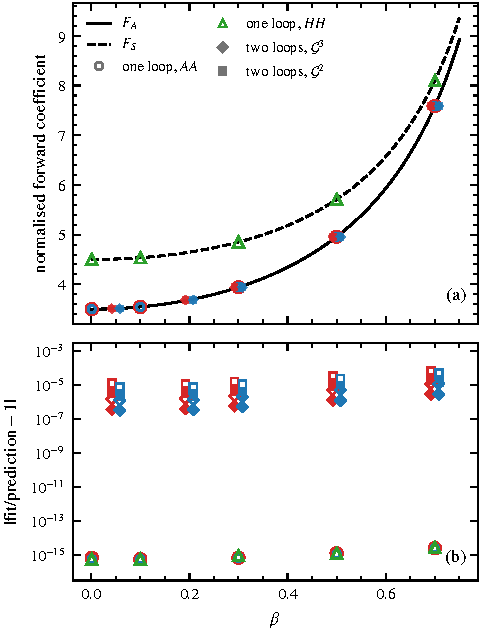
\includegraphics[width=\columnwidth]{figures/fig7_dps.pdf}
 \caption{Forward coefficients and helicity weights. (a) Circles: $D(\beta)$ for $gg\to AA$, Eq.~\eqref{eq:dps-prediction}, for $(\Nc,\nf)=(3,5)$ (red, large) and $(4,2)$ (blue, small), which coincide. Triangles: $-D(\beta)$ for $gg\to HH$ through two CP-even effective vertices at $(\Nc,\nf)=(3,5)$; the sign reversal accounts for the relative sign of the scalar and pseudoscalar tree amplitudes at threshold. Filled diamonds and squares: the coefficients of $\mathcal G^3$ and $\mathcal G^2$ in the forward limit of the two-loop remainder of $gg\to AA$, divided by $-\tfrac43\Nc\cdot2\pi\Nc m^2$ and $-2\beta_0\cdot2\pi\Nc m^2$ (Sec.~\ref{sec:two-loop}), for the same two sets (red and blue, drawn side by side). Solid and dashed curves: $F_A((1+\beta)/2)$ and $F_S((1+\beta)/2)$. (b) Relative deviations from these predictions; for the two-loop coefficients, filled symbols are fits over $1-c=10^{-7},\ldots,10^{-10}$ and open symbols include $1-c=10^{-6}$.}
 \label{fig:dps}
\end{figure}

\paragraph{Colour, scale dependence and phase.}

The factorisation also explains the flavour
and colour dependence of the one-loop
logarithm. The $O_G$ vertices couple only
to gluons, so only gluon splittings enter this
singular configuration and its coefficient is
independent of $\nf$. The factor $\Nc$
comes from the colour contraction of
the two three-gluon vertices.
Renormalisation and IR subtraction
do not change this logarithmic coefficient:
at one loop, their contributions are
proportional to the tree amplitude and
do not generate a logarithm of $p_T$.
The coefficient is therefore independent
of $\muR$.

Finally, the coefficient
$\OneLoopAone\,\mA^2$ of $\mathcal L$ is
real, whereas
$\mathcal M_1^{(0)}\to2i\mA^2$
at threshold. The logarithm is thus
out of phase with the tree amplitude
by $90^\circ$.
This relative phase is consistent
with the absorptive origin of the
one-loop DPS singularity, which can
be obtained from cuts that put
internal lines on
shell~\cite{GauntStirling2011}.
It explains why the one-loop DPS
logarithm does not contribute to
the interference with the tree
amplitude, as discussed in
Sec.~\ref{sec:rate}.

\subsection{Two loops}
\label{sec:two-loop}

The leading logarithms of the calculated two-loop coefficient $\mathcal M_1$ can be written in terms of the one-loop DPS logarithm. Comparing the coefficients of Eq.~\eqref{eq:leading-coefficients} with the coefficient $\OneLoopAone$ of Eq.~\eqref{eq:one-loop-threshold} gives, for general $\Nc$ and $\nf$,
\begin{equation}
 \widehat A_{13}\mathcal L^3+\widehat A_{12}\mathcal L^2
 =\OneLoopAone\,\mathcal L\left[\LogRelationCubic\,\mathcal L^2-2\beta_0\,\mathcal L\right],
 \label{eq:log-relation}
\end{equation}
with $\beta_0$ as in Eq.~\eqref{eq:normalisation}.
A similar relation holds in planar $\mathcal N=4$ super Yang--Mills theory.
Reference~\cite{DixonEsterlis2016} studied the six-gluon maximally
helicity violating (MHV) amplitude in planar $\mathcal N=4$ super
Yang--Mills theory, which has two negative and four positive helicities
when all momenta are outgoing. Near the configuration that mimics double
parton scattering, its singular terms obey an evolution equation, derived
following the analysis of crossing Wilson lines by Korchemskaya and
Korchemsky~\cite{KorchemskayaKorchemsky1995}, which fixes the leading
logarithms to all orders. The ratio of the leading two-loop and one-loop
terms, including their powers of the coupling, is $-(a/6)\ln^2\delta$,
where $a=g^2\Nc/(8\pi^2)$ and $\delta$, which measures the approach to the
singular configuration, is proportional to the squared transverse momentum
at fixed values of the other kinematic variables. With $a=2\Nc\as$ and
$\ln\delta=2\mathcal L+\mathrm{const}$, the ratio becomes
$-\tfrac43\Nc\as\mathcal L^2$ at leading logarithmic order. This is the
ratio of the cubic term in Eq.~\eqref{eq:log-relation} to the one-loop
logarithm, once the additional power of $\as$ at two loops is included.
The second term, $-2\beta_0\mathcal L$, has no counterpart in the
$\mathcal N=4$ theory; the number of quark
flavours enters it only through $\beta_0$.


The same $\beta_0$ term appears in the NLO momentum-space kernel for the
splitting $g\to gg$ in unpolarised colour singlet double parton
distributions~\cite{Diehl:2019rdh}, in which the transverse momentum
mismatch $\Delta$ between amplitude and conjugate amplitude plays the role
of $p_T$. Equations~(50) and (135) of Ref.~\cite{Diehl:2019rdh} give the
coefficient of $\ln^2(\mu^2/\Delta^2)$ in units of $\alpha_s/2\pi$;
relative to the LO term, its $\beta_0$ part corresponds to
$-2\beta_0\mathcal L$ in the normalisation of $\as$ used here. Half of it
comes from the renormalisation of the coupling and half from the
$\delta$-function parts of the DGLAP kernels, so that the running of the
coupling alone would give $-\beta_0\mathcal L$. The other terms of the
kernel have no counterpart in the amplitude: a term proportional to
$C_A\ln[x(1-x)]$ from the plus distributions, which contributes where the
two momentum fractions add up to one, and the real emission terms, which
contribute where they add up to less than one.


The relation of Eq.~\eqref{eq:log-relation} is not restricted to threshold. In the forward limit at fixed velocity a convenient variable is $\mathcal G=\tfrac12\ln[(\mA^4-tu)/\mA^4]=\mathcal L-\ln(1-\bA^2)$, in which the one-loop DPS logarithm is $C_1\mathcal G$ with $C_1=2\pi\Nc m^2F_A\bigl((1+\beta)/2\bigr)$, by Eq.~\eqref{eq:dps-prediction}. In this limit the two-loop logarithms of the threshold series are exactly $C_1\bigl[-\tfrac43\Nc\,\mathcal G^3-2\beta_0\,\mathcal G^2\bigr]$ through $\bA^6$, for general $\Nc$ and $\nf$; at fixed angle, the coefficient of $\mathcal L^3$ follows the expansion of $F_A\bigl((1+\bA)/2\bigr)$ order by order. Away from threshold I evaluated the released two-loop remainder of $\mathcal M_1$ at $1-c=10^{-6},\ldots,10^{-10}$ with \MoneFwdDigits-digit arithmetic, checked with \MoneFwdCheckDigits{} digits, which agree to at least \MoneFwdCheckAgreement{} digits, and fitted a cubic polynomial in $\ln(1-c)$. For $\MoneFwdBetaMin\leq\beta\leq\MoneFwdBetaMax$ and $(\Nc,\nf)=$ \MoneFwdSets, the coefficients of $\mathcal G^3$ and $\mathcal G^2$ agree with this form to \MoneFwdDevThree{} and \MoneFwdDevTwo{}, with imaginary parts below \MoneFwdImag{} of their magnitudes, when the point at $1-c=10^{-6}$ is left out; with it, the deviations are about \MoneFwdWindowFactor{} times larger, as expected from power corrections in $1-c$ (Fig.~\ref{fig:dps}). In the forward limit, the two-loop leading logarithms of $\mathcal M_1$ are therefore the one-loop DPS logarithm, with its helicity weight $F_A(x)$, multiplied by the same factor at every velocity tested.

The $|J_z|=2$ amplitude acquires a logarithm at two loops: the term
$\widehat A_{22}\mathcal L^2$, with
$\widehat A_{22}=(\MtwoRelation)\cdot\OneLoopMtwo$, is the one-loop
constant multiplied by $\MtwoRelation\,\mathcal L^2$. The forward-limit calculation described next indicates that the same coefficient relation persists away from threshold. In the forward limit $c\to1$ at fixed velocity, where $p_T\to0$ as well, I evaluated the released two-loop remainder of $\mathcal M_2$ at $1-c=$ \JzExponents{} with \JzDigits-digit arithmetic and fitted a quadratic polynomial in $\ln(1-c)$; a repetition with \JzCheckDigits{} digits agrees to at least \JzCheckAgreement{} digits. For $\JzBetaMin\leq\beta\leq\JzBetaMax$ and $(\Nc,\nf)=$ \JzSets, the real part of the coefficient of $\ln^2(2p_T/m)$ equals $-4\Nc$ times the forward limit of $\mathcal M_2^{(1)}$ to \JzMaxDev, although that limit varies by a factor of \JzKOneRatio{} over this range. Its imaginary part, which should vanish, is below \JzImag{} of its magnitude, and including the point at $1-c=10^{-4}$ in the fit increases the deviation to \JzMaxDevWide, as expected from power corrections. Within the range tested, the one-loop amplitude and the fitted two-loop logarithm are therefore consistent with
\begin{equation}
 \as\mathcal M_2^{(1)}\bigl[1-4\Nc\as\ln^2(2p_T/m)\bigr],
 \label{eq:jz2-forward}
\end{equation}
with no additional velocity or flavour dependence resolved in the coefficient of the double logarithm.


The observed combination has the form of the expansion of
$\exp(-4\Nc\as\mathcal L^2)$ to first order in $\as$. Multiplied by the one-loop coefficient $\OneLoopAone$ and
integrated over $\mathcal L$, the same exponential gives the cubic term of
Eq.~\eqref{eq:log-relation}. At lowest order it also corresponds to the
factor $\exp(-\gamma_K\ln^2\delta/8)$ of Ref.~\cite{DixonEsterlis2016},
with the cusp anomalous dimension $\gamma_K=4a$. However, two loops cannot
decide whether this factor exponentiates in QCD. The $J_z$ argument of
Sec.~\ref{sec:dps} concerns the one-loop singularity and does not forbid
this logarithm. Nor can it come from two-loop amplitudes of the
subprocesses, since conservation of angular momentum forbids $gg\to A$ for
opposite gluon helicities to all orders; its dynamical origin remains open. A related
effect occurs in planar $\mathcal N=4$ super Yang--Mills theory. The
next-to-MHV (NMHV) six-gluon amplitude, with three negative helicities, has
no such singularity at one loop because of $J_z$ conservation, but Dixon
and Esterlis found logarithmic singularities starting at two loops, in the
region where the limit overlaps with multi-Regge kinematics, and suggested
that they may come from contributions in which more than one particle
crosses a cut~\cite{DixonEsterlis2016}.

The forward limit of $\mathcal M_2^{(1)}$ itself has a closed form. The exact one-loop remainders agree with
\begin{equation}
 \lim_{c\to1}\frac{\mathcal M_2^{(1)}}{m^2}=\pi\Nc\,\frac{x^4+(1-x)^4}{x(1-x)},\qquad x=\frac{1+\beta}{2},
 \label{eq:K1}
\end{equation}
to \KOneClosedDev{} for $\KOneBetaMin\leq\beta\leq\KOneBetaMax$ and both sets of $(\Nc,\nf)$; at threshold it gives $\OneLoopMtwo$. With the weights of Eq.~\eqref{eq:splitting-weights}, the fraction in Eq.~\eqref{eq:K1} equals $w_{+-}(x)w_{-+}(1-x)+w_{-+}(x)w_{+-}(1-x)$: the helicity sum of Sec.~\ref{sec:dps} for the two pairings that an opposite-helicity initial state allows when each effective vertex receives two gluons of equal helicity, with the same overall factor $\pi\Nc$ as in Eq.~\eqref{eq:dps-prediction}. The one-loop constant of $\mathcal M_2$ thus has the form expected if it arose from the DPS region, where the azimuthal phase of these pairings removes the logarithm and leaves a finite term; I have not derived this from the factorisation formula. The two helicity amplitudes therefore provide an explicit two-loop QCD benchmark for a more general description of this singular kinematic region.


%
Figure~\ref{fig:amplitudes} compares the three orders. With $\as=\BenchAs$ ($\alpha_s=\BenchAlphaS$), at $\bA=\LoopSizeBeta$ and $c=\BenchCos$, the one and two-loop terms of $\mathcal M_1$ are \MoneOneLoopRatio{} and \MoneTwoLoopRatio{} times the tree term, and the one-loop term of $\mathcal M_2$ is \MtwoOneLoopRatio{} times the tree term. The last ratio grows as $\bA^{-2}$ towards threshold, since the tree-level $|J_z|=2$ amplitude vanishes there. The one-loop terms include the scale term of Eq.~\eqref{eq:normalisation}. Towards threshold, the loop terms of $\mathcal M_1$ grow with $|\mathcal L|$, the two-loop term as $|\mathcal L|^3$ and the one-loop term as $|\mathcal L|$, so that below $\bA\approx\CrossoverBeta$ the two-loop term exceeds the one-loop term at this angle. Because the logarithms are out of phase with the tree amplitude, this growth largely drops out of the cross section (Sec.~\ref{sec:rate}). In panel (b) the one-loop term of $\mathcal M_2$ tends to the constant of Eq.~\eqref{eq:one-loop-threshold}, while the two-loop term grows as $\mathcal L^2$, the logarithm that the $|J_z|=2$ amplitude acquires at two loops.
%

\section{Consequences for the cross section}
\label{sec:rate}

\subsection{Leading order}

Averaging Eq.~\eqref{eq:helicity} over helicities and colours, and including a factor $\tfrac12$ for identical particles, gives the LO partonic cross section of the Type~II amplitude,
\begin{equation}
 \frac{\dd\hat\sigma}{\dd c}
 =\frac{\bA\,C_G^4}{128\pi\hat s\,(\Nc^2-1)}\left(|\mathcal M_1^{(0)}|^2+|\mathcal M_2^{(0)}|^2\right)
 \label{eq:dsigma}
\end{equation}
for $-1<c<1$. For $\alpha_s=\BenchAlphaS$, $\cot\beta_H=\BenchCotBeta$ and $\mA=\BenchMA\,\mathrm{GeV}$ I find $\hat\sigma=\SigmaLO\,\mathrm{pb}$ at $\bA=\SigmaBeta$ (Fig.~\ref{fig:cross-section}(a)). The cross section rises as $\bA$ above threshold and as $\hat s$ at large $\hat s$, as expected for dimension-five operators, and it is of fourth order in $\as$ through $C_G^4$. In a 2HDM, it is a small part of the total, which is dominated by Type~I (Sec.~\ref{sec:counting}).
%
\begin{figure*}[t]
 \centering
 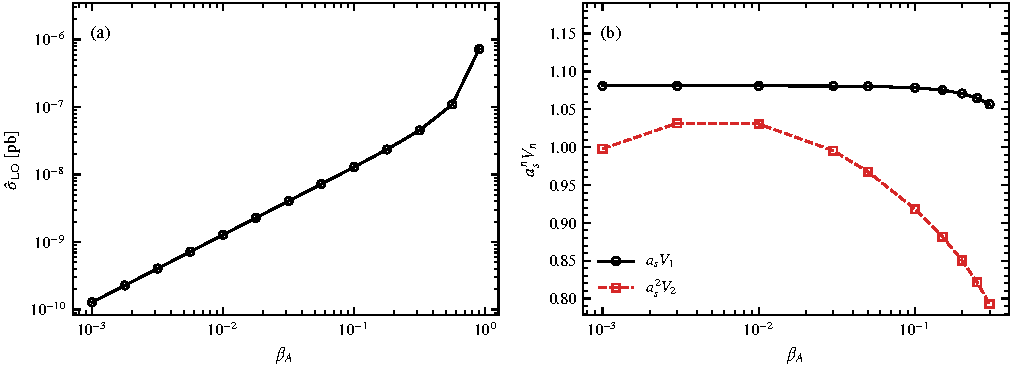
\includegraphics[width=0.94\textwidth]{figures/fig6_cross_section.pdf}
 \caption{(a) Leading order partonic cross section of the Type~II amplitude, Eq.~\eqref{eq:dsigma}, for $\mA=\BenchMA\,\mathrm{GeV}$, $\alpha_s=\BenchAlphaS$ and $\cot\beta_H=\BenchCotBeta$. (b) Finite virtual corrections of Eq.~\eqref{eq:virtual}, averaged over the angle, for $\muR=\mA$, $\Nc=\BenchNc$ and $\nf=\BenchNf$.}
 \label{fig:cross-section}
\end{figure*}

\subsection{Finite virtual corrections}

To examine the effect of the loop corrections on the Type~II squared amplitude, I define two dimensionless
coefficients, $V_1$ and $V_2$, relative to the tree contribution. Let $\mathcal A_{\Fin}$ denote the
amplitude constructed from the finite remainders of Eq.~\eqref{eq:catani}, in the normalisation of
Eq.~\eqref{eq:normalisation}. Using the helicity decomposition in Eq.~\eqref{eq:helicity}, its square
can be written as
\begin{align}
 \sum_{\mathrm{hel,col}}|\mathcal A_{\Fin}|^2
 &=2(\Nc^2-1)\,C_G^4
   \sum_i|\mathcal M_i^{(0)}|^2
 \nonumber\\
 &\quad\times
 \left[1+\as V_1+\as^2V_2+\Ord(\as^3)\right],
 \nonumber\\
 V_1
 &=\frac{
  2\Real\sum_i
  \mathcal M_i^{(0)*}\mathcal M_i^{(1)}
 }{
  \sum_i|\mathcal M_i^{(0)}|^2
 },
 \nonumber\\
 V_2
 &=\frac{
  \sum_i\left(
   2\Real\bigl[\mathcal M_i^{(0)*}\Mfull{i}\bigr]
   +|\mathcal M_i^{(1)}|^2
  \right)
 }{
  \sum_i|\mathcal M_i^{(0)}|^2
 }.
 \label{eq:virtual}
\end{align}
The sums run over the two tensor coefficients, $i=1,2$. The coefficient $V_1$ contains the
interference between the tree and one-loop amplitudes. At the next order, $V_2$ contains
both the interference between the tree and two-loop amplitudes and the square of the
one-loop amplitude.

These coefficients refer only to the $O_G$--$O_G$ Type~II contribution. Their
interpretation as NLO and NNLO finite virtual terms applies when the Type~II
tree amplitude is the leading amplitude, as for a pseudoscalar coupled to gluons
only through $G\tilde G$ (Sec.~\ref{sec:counting}). They do not
include interference with the Type~I amplitudes present in a 2HDM.

The quantities $V_1$ and $V_2$ depend on the subtraction scheme of
Eq.~\eqref{eq:catani}; they are not observables or $K$ factors. A physical
cross section requires the virtual and
real emission contributions to be combined consistently with the
counterterms for initial state collinear factorisation. The real
emission contributions are not included here.
%
At fixed $\bA$, both coefficients depend on the scattering angle. To display
their velocity dependence in Fig.~\ref{fig:cross-section}(b), I
average them over the angle using
the Type~II LO cross section as the weight:
\begin{equation}
 \langle V_n\rangle
 =
 \frac{
  \displaystyle
  \int_{-1}^{1}\dd c\,
  \sum_i|\mathcal M_i^{(0)}|^2\,V_n
 }{
  \displaystyle
  \int_{-1}^{1}\dd c\,
  \sum_i|\mathcal M_i^{(0)}|^2
 },
 \qquad n=1,2.
 \label{eq:angle-average}
\end{equation}
At fixed $\bA$, the remaining factors in Eq.~\eqref{eq:dsigma} are independent
of $c$ and cancel in this ratio. Thus, $\as\langle V_1\rangle$ and
$\as^2\langle V_2\rangle$ give the finite virtual contributions relative
to the angularly integrated tree contribution, rather than an
unweighted average of the corrections.
The integrals are evaluated with \QuadNodes-point Gauss--Legendre quadrature in $c$; with \QuadNodesRef{} points, $\langle V_1\rangle$ changes by less than \QuadVoneDev{} and $\langle V_2\rangle$ by less than \QuadVtwoDev{} relative to its value at $\bA=$ \QuadBetas{}.

I evaluate the one-loop remainders without a threshold expansion and
use the series through $\bA^6$ for the two-loop remainders.
For $\alpha_s=\BenchAlphaS$ and $\muR=\mA=\BenchMA\,\mathrm{GeV}$,
$\as\langle V_1\rangle$ lies between
\VoneMin{} and \VoneMax{}, while $\as^2\langle V_2\rangle$ lies between
\VtwoMin{} and \VtwoMax{} over $\VirtualBetaMin\leq\bA\leq\VirtualBetaMax$.
These are the two curves shown in
Fig.~\ref{fig:cross-section}(b).
At fixed kinematics, the scale dependence of the one-loop remainder
in Eq.~\eqref{eq:normalisation} implies $\partial V_1/\partial\ln\muR^2=4\beta_0$.

\paragraph{One-loop contribution.}

The threshold behaviour of $V_1$ and $V_2$ follows from the relative phases of the tree and loop
amplitudes. At fixed scattering angle, $\mathcal M_1^{(0)}\to2i\mA^2$, whereas
$\mathcal M_2^{(0)}$ vanishes as $\bA^2$.
The squared tree amplitude in the denominator of Eq.~\eqref{eq:virtual} therefore tends to
$4\mA^4$. At leading power, interference with the tree amplitude selects the imaginary part
of $\mathcal M_1^{(1)}$ or $\Mfull{1}$.

To separate the real logarithm from the constant phase, define
\[
 \ell=\ln\frac{2p_T}{\mA},
 \qquad
 \mathcal L=\ell+\frac{i\pi}{2}+\Ord(\bA^2),
\]
where the second relation follows from Eq.~\eqref{eq:calL}. At leading power, the
one-loop result in Eq.~\eqref{eq:one-loop-threshold} is
\[
 \frac{\mathcal M_1^{(1)}}{\mA^2}
 =
 \OneLoopAone\,\ell
 +\frac{i\pi}{2}\OneLoopAone
 +\widehat A^{(1)}_{10}.
\]
The coefficient of $\ell$ is real, so this term does not interfere with the imaginary
tree amplitude. The imaginary constant terms do contribute, giving
\begin{equation}
 V_1\longrightarrow
 \frac{\pi}{2}\OneLoopAone
 +\Imag\widehat A^{(1)}_{10}.
 \label{eq:v1-threshold}
\end{equation}
For $\Nc=\BenchNc$, $\nf=\BenchNf$ and
$\muR=\mA$, this gives
$V_1\to\VoneThreshold$.
Thus, the one-loop remainder contains a DPS logarithm, but the leading power
finite virtual correction does not. Its limiting value is independent of the
angle, which explains why the angular average in Fig.~\ref{fig:cross-section}(b)
is nearly constant.

\paragraph{Two-loop contribution.}

At the next order, the interference of the two-loop amplitude with the tree amplitude again selects the imaginary part of the loop remainder. The square of the one-loop amplitude, however,
retains the real logarithm. Using Eqs.~\eqref{eq:leading-power} and
\eqref{eq:one-loop-threshold}, the leading power terms of
Eq.~\eqref{eq:virtual} can be written as
\begin{align}
 V_2\big|_{\bA^0}
 &=
 \Imag\left[
  \sum_{k=0}^{3}\widehat A_{1k}\mathcal L^k
 \right] +
 \frac14\left|
  \OneLoopAone\,\mathcal L
  +\widehat A^{(1)}_{10}
 \right|^2
 +\frac{\pi^2\Nc^2}{16}.
\end{align}
The first term is the interference of the two-loop amplitude with the tree amplitude, and the second is the square of $\mathcal M_1^{(1)}$. The last term comes from $|\mathcal M_2^{(1)}|^2$,
since $\mathcal M_2^{(1)}\to\pi\Nc\mA^2/2$. It contributes at leading power even
though the corresponding tree amplitude vanishes. By contrast, interference
between $\mathcal M_2^{(0)}$ and $\Mfull{2}$ is suppressed by $\bA^2$,
up to logarithms.

The coefficients $\widehat A_{13}$ and $\widehat A_{12}$ are real. At leading power,
\[
 \Imag\mathcal L^3
 =\frac{3\pi}{2}\ell^2-\frac{\pi^3}{8},
 \qquad
 \Imag\mathcal L^2=\pi\ell.
\]
Consequently, the cubic logarithm of the two-loop amplitude gives a quadratic,
not a cubic, logarithm in its interference with the tree amplitude. The term
$\widehat A_{12}\mathcal L^2$ contributes only a linear logarithm to this
interference. The square of the one-loop amplitude is also at most
quadratic in $\ell$.

The leading threshold expansion of $V_2$ therefore has the form
\begin{equation}
 V_2=v_0+v_1\ell+v_2\ell^2
     +\Ord_{\log}(\bA^2).
 \label{eq:v2-form}
\end{equation}
Here $v_0$, $v_1$ and $v_2$ are the coefficients of the constant, linear
and quadratic terms in $\ell$. They all belong to the same
perturbative coefficient $V_2$; their subscripts do not count loops.

The coefficient $v_2$ receives two contributions.
The interference of the two-loop amplitude with the tree amplitude gives
$\tfrac32\pi\widehat A_{13}
=-14\pi^2\Nc^2$, while the square
of the one-loop amplitude gives
$\tfrac14(\OneLoopAone)^2
=\tfrac{49}{4}\pi^2\Nc^2$.
Their sum is
\begin{equation}
 v_2
 =-14\pi^2\Nc^2+\frac{49}{4}\pi^2\Nc^2
 =-\frac74\pi^2\Nc^2.
 \label{eq:v2-log}
\end{equation}
The two terms partly cancel, with the negative interference contribution
larger in magnitude. At leading power, the DPS logarithm thus first appears
in the finite virtual correction through $V_2$, where its highest
power is $\ell^2$.

A fit of the numerical values of $V_2$ at $c=\BenchCos$ over
$\VtwoBetaSmall\leq\bA\leq\VtwoBetaLarge$ gives $v_2=\VtwoLogFit$.
Equation~\eqref{eq:v2-log} gives $\VtwoLogExact$ for $\Nc=\BenchNc$;
the relative difference before rounding is \VtwoLogRelDiff{}. For $\as=\BenchAs$, the quadratic term
in the finite virtual correction is $\as^2v_2\ell^2=\VtwoLogScaled\,\ell^2$.

\paragraph{Remaining coefficients and numerical behaviour.}

At leading power, $v_0$, $v_1$ and $v_2$ are independent of the scattering
angle. The angular dependence of $V_2$ itself remains through $\ell$.
Fits for $v_0$ and $v_1$ at $c=0$, $\tfrac13$ and $\tfrac23$
agree within a relative spread of \VtwoAngleSpread{}.
The coefficient of the linear logarithm follows from the same expansion:
\begin{align*}
 v_1
 &=\pi\widehat A_{12}
   +\Imag\widehat A_{11}
   +\frac{\OneLoopAone}{2}
    \Real\widehat A^{(1)}_{10}
 \\
 &=\frac72\pi\Nc\Real\widehat A^{(1)}_{10}
   +7\pi^2\Nc\beta_0.
\end{align*}
For the benchmark parameters, this gives $v_1=\VoneFit$, in agreement with
the numerical fit to a relative difference of \VoneFormulaDev{}.
The coefficient is independent of $\muR$, since
$\Real\widehat A^{(1)}_{10}$ is scale independent. The same is true
of $v_2$. At leading power, the explicit scale dependence of $V_2$
is therefore confined to $v_0$, hich changes from \VzeroBench{}
to \VzeroTwoMu{} when $\muR$ is increased from $\mA$ to $2\mA$.

Although $\ell^2$ is the highest power of the logarithm, it need
not give the largest contribution at the velocities considered.
At $c=\BenchCos$, the ratio $(v_1\ell+v_2\ell^2)/V_2$ is
approximately \LogShareLarge\% at $\bA=\LogShareBetaLarge$
and \LogShareSmall\% at $\bA=\LogShareBetaSmall$.
The quadratic term alone contributes $-\SquareShareLarge\%$ and
$-\SquareShareSmall\%$ of the total $V_2$, respectively.
Since $\ell<0$ in this region and both $v_1$ and $v_2$ are
negative, the linear term is positive and the quadratic term is negative.
%
This competition also explains the shape of the correction as a
function of velocity. The leading power expression has a maximum at
\[
 \ell_{\mathrm{max}}
 =-\frac{v_1}{2v_2}
 =\VtwoPeakEll.
\]
At $c=\BenchCos$, this corresponds to $\bA\simeq\VtwoPeakBeta$.
For larger $\bA$, $\ell$ increases and the leading power value of
$V_2$ decreases. The same balance between the linear and quadratic
terms explains the turnover of the angular average
$\as^2\langle V_2\rangle$ in Fig.~\ref{fig:cross-section}(b).
At $c=\BenchCos$ and $\bA=\LogShareBetaLarge$,
including the terms beyond leading power changes $V_2$ by only \LeadPowerDevLarge\%.

\paragraph{DPS interpretation and subtraction dependence.}

The two contributions to $v_2$ also differ in their relation to the DPS
configuration. In the square of the one-loop amplitude, the DPS
region occurs in both the amplitude and its complex conjugate, that is,
on both sides of the final state cut. This is the configuration
associated with perturbative splittings in both protons that
overlaps with DPS and requires a subtraction to avoid double
counting~\cite{DiehlGauntSchoenwald2017,DiehlPloessl2026}.
In the interference with the tree amplitude, the DPS region occurs
only on the loop side of the cut. Both contributions enter the
finite virtual coefficient $V_2$ defined in Eq.~\eqref{eq:virtual}; the
logarithmic term in its one-loop square alone would therefore
not give the complete coefficient $v_2$.

Although $V_2$ depends on the IR subtraction convention, $v_2$ is unchanged by finite
scheme changes that multiply lower order amplitudes by angle independent functions
regular at the pair threshold. The tree amplitude has no
logarithm, and the one-loop remainder contains at most one power of $\ell$. Such changes can therefore
affect the constant and linear terms in $V_2$, but not the coefficient of $\ell^2$.

Finally, with the Wilson coefficient counting specified in
Sec.~\ref{sec:counting}, the one-loop $O_G$--$O_J$ amplitude contributes
at the same order as the two-loop $O_G$--$O_G$ amplitude.
Its coefficient $C_J$ depends on $m_t$ in the heavy top quark
theory~\cite{Bhattacharya:2019bmd}. By Eq.~\eqref{eq:gj-proportional},
the mixed amplitude is proportional to the tree amplitude. After
including its Wilson coefficient and matching the normalisation,
its interference with the tree amplitude therefore gives a
kinematically constant shift to $V_2$. It changes $v_0$,
but not $v_1$ or $v_2$, and is not included in the results above.


\subsection{Use in higher order calculations}
\label{sec:use}

The threshold series provide a compact representation of the two-loop Type~II finite remainders near the
pair production threshold. For the two-body virtual amplitude, $m_{AA}=\sqrt{\hat s}$, and
\[
 \frac{m_{AA}}{2\mA}
 =\frac{1}{\sqrt{1-\bA^2}}.
\]
The range $\bA\leq\RecommendedBeta$ therefore corresponds to pair invariant masses up to
$\ThresholdPercentPointTwo\%$ above $2\mA$. For $\mA=\BenchMA\,\mathrm{GeV}$, the upper limit
is $m_{AA}=\SqrtSPointTwo\,\mathrm{GeV}$. The point $\bA=\EdgeBeta$ lies
$\ThresholdPercentPointThree\%$ above threshold.

I recommend the series through $\bA^6$ for $0<\bA\leq\RecommendedBeta$ at the angles tested
in Tables~\ref{tab:validation-grid} and \ref{tab:forward-angles}.
At $\bA=\EdgeBeta$, the largest relative error
of the complete coefficients on the validation grid is \PtwoErrAtPointThree{}.
These numerical checks do not establish a uniform accuracy bound as $c\to\pm1$, where
the logarithms diverge. The series retain the complex values of both tensor coefficients,
including the phases needed for interference with other amplitudes. Such contributions
must be combined using the same normalisation, Wilson coefficient conventions, tensor basis
and infrared subtraction scheme.

One application is the calculation of the hard function for a threshold resummed or
soft-virtual prediction of the pair invariant mass distribution. In this context, threshold
refers to the limit in which little energy is available for additional QCD radiation
at fixed $m_{AA}$, rather than to the pair
production limit $\bA\to0$~\cite{Sterman:1986aj,Catani:1989ne,deFlorian:2015moa}.
At leading power in the soft limit, the soft and collinear factors are universal
for gluon fusion into a colour singlet final state. The process dependence enters
through the finite virtual contributions to the hard function~\cite{deFlorian:2012za,Bhattacharya:2021nsv}.
The hard function is therefore needed at each pair invariant mass, and the present
series provide its two-loop Type~II amplitude input near $m_{AA}=2\mA$.

To construct this contribution, the finite remainders must first be combined with
the appropriate lower order amplitudes. When the Type~II tree amplitude is the
leading amplitude, the relevant $O_G$--$O_G$ combinations are those in
Eq.~\eqref{eq:virtual}. In particular, the NNLO virtual term contains both the
interference of the two-loop amplitude with the tree amplitude and the square
of the one-loop amplitude. Integrated over the scattering angle at fixed $m_{AA}$ and
divided by the integrated tree contribution, they give the averages of
Eq.~\eqref{eq:angle-average}. The finite virtual terms must then
be combined with the universal contributions according to the
subtraction and resummation conventions of the chosen calculation~\cite{deFlorian:2012za}.
For Higgs pairs, Ref.~\cite{deFlorian:2015moa} gives an explicit construction in which
the two-loop finite virtual contribution is integrated over $t$ at fixed pair invariant mass.

The perturbative order of the present contribution depends on the leading
amplitude, as explained in Sec.~\ref{sec:counting}.
For a pseudoscalar coupled to gluons only through $G\tilde G$, the two-loop
Type~II remainders enter the NNLO virtual contribution. In a 2HDM, they first contribute at
N$^3$LO through interference with the leading Type~I amplitude.
In that case, the Type~II angular averages of Eq.~\eqref{eq:angle-average}
cannot be used directly: the interference with Type~I must be formed before the
angular integration. The remaining amplitudes and any mixed $O_G$--$O_J$ contribution must
also be included at the order required by the theory. For Higgs pairs, likewise,
the NNLO virtual corrections contain the diagrams with two effective vertices only
at tree level and at one loop~\cite{deFlorianMazzitelli2013Virtual},
and their two-loop terms are an ingredient of N$^3$LO~\cite{Banerjee:2018lfq}.

\section{Conclusions}
\label{sec:conclusions}

I have expanded the two-loop Type~II finite remainders
for $gg\to AA$ with two $O_G$ insertions about the
pair production threshold through $\bA^6$ at fixed
scattering angle. After the endpoint constants are
expressed in a basis of \BasisCountWord{}
transcendental constants, all inverse powers of
$\bA$ and the odd powers through $\bA^5$ cancel
identically. Every coefficient is even in
$\cos\theta$, as required by Bose symmetry.
For $0<\bA\leq\RecommendedBeta$, the maximum
relative errors of the two complete coefficients
are \PoneErrLePointTwo{} and
\PtwoErrLePointTwo{}, respectively, at the
points tested, including the forward angles.
The released series files are a factor of
\SizeRatio{} smaller than the expressions
released with Ref.~\cite{Bhattacharya:2019bmd}.
The timing comparisons in
App.~\ref{app:data} also show faster evaluation
for the representations tested.

A consistent comparison of the perturbative orders also required
converting the remainders of Ref.~\cite{Bhattacharya:2019bmd} to a common normalisation. The two-loop files carry an
overall factor of \FileFactor{} relative to
the tree and one-loop amplitudes, and the
one-loop files are given at $\muR=1$~GeV.
After the scale dependence is added and
all orders are brought to a common normalisation, the
remainders satisfy the renormalisation group
relations in Eqs.~\eqref{eq:rg-one} and
\eqref{eq:rg-two} within the accuracy of
the checks described in
App.~\ref{app:normalization}.
The Ref.~\cite{Bhattacharya:2019bmd} pole cancellation is unaffected, since all terms of the two-loop subtraction
carry the same overall factor.

At leading power, the angular dependence
enters entirely through the logarithm of
the transverse momentum of the pseudoscalars.
I identified the one-loop logarithm with
the DPS singularity studied in
Ref.~\cite{GauntStirling2011}.
The gluon splitting weights and the
relative signs of the CP-odd subprocess
amplitudes determine the momentum fraction
dependence of its coefficient.
With the overall constant fixed at
threshold, the resulting expression
reproduces the velocity dependence
of the exact one-loop coefficient
in the forward limit to a relative
accuracy of \DPSMaxDeviation{} over
the tested range.
The same analysis explains the absence
of a one-loop logarithm in the
$|J_z|=2$ amplitude, the independence
of the logarithmic coefficient from
$\nf$ and $\muR$, and its phase relative
to the tree amplitude.
An explicit one-loop calculation of
$gg\to HH$ through two CP-even vertices
confirms the corresponding scalar
weight $F_S$, using the normalisation
fixed from $AA$ and accounting for
the relative sign of the tree
amplitudes. The opposite helicity
amplitude again has no one-loop
DPS logarithm.

At two loops, the $J_z=0$ amplitude
grows as $\ln^3p_T$ and the
$|J_z|=2$ amplitude as $\ln^2p_T$.
The ratio of the leading two-loop
and one-loop logarithms in the
$J_z=0$ amplitude agrees with the
corresponding ratio in the all-orders
result for planar $\mathcal N=4$
super Yang--Mills
theory~\cite{DixonEsterlis2016}.
The coefficient of the quadratic
logarithm in this amplitude is
proportional to $\beta_0$, with
the structure discussed in
Sec.~\ref{sec:two-loop} in relation
to the NLO $g\to gg$ splitting
kernel for double parton
distributions~\cite{Diehl:2019rdh}.
The finite virtual corrections
are less singular than the
amplitudes. At leading power,
the one-loop DPS logarithm does
not contribute to $V_1$, because
it is out of phase with the
tree amplitude. The cubic
logarithm is absent from $V_2$,
whose highest logarithmic term is
\[
 V_2\supset
 -\frac74\pi^2\Nc^2
 \ln^2\!\left(\frac{2p_T}{\mA}\right).
\]
This coefficient results from a
partial cancellation between the
interference of the two-loop amplitude
with the tree amplitude and the square
of the one-loop amplitude.

Several questions remain open. The overall factor $\pi\Nc m^2$ multiplying the one-loop helicity weight has not yet been derived directly from the factorisation formula with the effective vertices. At two loops, a general treatment of the singular region would have to reproduce the different logarithmic powers of the $J_z=0$ and $|J_z|=2$ amplitudes, their colour and flavour dependence, and the reduction of the singularity in the finite virtual correction. In the forward limit, the two-loop logarithms of the $J_z=0$ amplitude follow the one-loop helicity weight at all velocities tested, and fits give numerical evidence that the real coefficient of the $|J_z|=2$ double logarithm is $-4\Nc$ times the one-loop forward amplitude, which itself has the closed form of Eq.~\eqref{eq:K1}; the mechanism producing this term has not been derived. The present results therefore provide explicit two-loop QCD benchmarks for such an analysis.
The known two-loop amplitudes for
$gg\to HH$ through two effective
vertices~\cite{Banerjee:2018lfq}
also permit a comparison with
the scalar case.
Finite top quark mass effects
are a separate question.
If the one-loop DPS factorisation
applies to the full theory, the
on-shell triangle form factors
in Eq.~\eqref{eq:top-dps} multiply
the logarithmic coefficient by
\TopMassDPSA{} at
$\mA=\TopMassMAA$~GeV.
This estimate does not determine
the mass dependence of the
remaining one-loop terms or the two-loop amplitude.

The series provide the two-loop Type~II amplitude input to the hard
function for the pair invariant mass distribution near $m_{AA}=2\mA$.
They enter at NNLO when the Type~II tree amplitude is the leading
amplitude, as for a pseudoscalar coupled to gluons only through
$G\tilde G$, and at N$^3$LO in a 2HDM, through interference with the
leading Type~I amplitude; Sec.~\ref{sec:use} describes how they are
combined with the other contributions. The mixed $O_G$--$O_J$
contribution, omitted from the numerical results for $V_2$, gives a
kinematically constant shift and leaves the logarithmic coefficients
unchanged. The series, the evaluator, the validation records and the code
of the construction are provided with the paper~\cite{SupplementalMaterial}.


\section*{Data Availability}

The threshold series, construction files, validation records, evaluator and the scripts that reproduce all tables and figures are provided as ancillary files with the arXiv version of this article and as Supplemental Material~\cite{SupplementalMaterial}. The unexpanded finite remainders used as input were published with Ref.~\cite{Bhattacharya:2019bmd}.


\begin{acknowledgments}
I thank IFIC, University of Valencia, and Prof.\ Francisco
Campanario for providing the computing resources used in
this work. I used large language models, Claude Opus 5.5 and Claude Fable 5.1 (Anthropic) and GPT-6 Pro and GPT-5.6 Pro (OpenAI), to help write and debug the code for the threshold construction, the validation and the figures, and to draft and edit the text. I specified each task and checked all code through the independent tests described in Secs.~\ref{sec:expansion} and~\ref{sec:physics} and App.~\ref{app:normalization}: comparison with the unexpanded remainders, the renormalisation group relations, and an independent Python evaluation. These tests are included in the released package. I am responsible for all results, their interpretation and the text.
\end{acknowledgments}

\appendix
\section{Endpoint constants}
\label{app:constants}

The boundary values of the expansion contain the constants
\begin{equation}
 \mathrm{MB}[p,q,a,w]
 =\frac{a}{(p-1)!}\int_0^1\dd t\,
 \frac{[-\ln t]^{p-1}}{1-at}\,\phi_q(wt),
 \label{eq:mb-definition}
\end{equation}
with $\phi_1(z)=-\ln(1-z)$ and $\phi_q(z)=\Li_q(z)$ for $q\geq2$. Besides the elementary values $\mathrm{MB}[2,2,1,1]=\pi^4/120$ and $\mathrm{MB}[2,1,1,1]=\zeta_3$, \ConstantCountWord{} distinct constants occur. They were evaluated by quadrature at high precision, independently of the amplitude data, and reduced to the basis of Eq.~\eqref{eq:constant-basis} with the PSLQ algorithm~\cite{Ferguson:1999} at \PSLQDigits{} digits. Table~\ref{tab:mb-constants} lists the results; the largest residual is \PSLQResidual, and the same relations were obtained in Mathematica.

\begin{table}[t]
\centering


\small
\begin{tabular}{cl}
\toprule
$[p,q,a,w]$ & reduction \\
\midrule
$[1,2,-1,1]$ & $- \frac{\pi^{2} \ln 2}{6} + \frac{5 \zeta_3}{8}$ \\
$[1,2,1/2,1/2]$ & $- \frac{\zeta_3}{4} - \frac{\ln^{3}2}{6} + \frac{\pi^{2} \ln 2}{12}$ \\
$[1,2,1/2,1]$ & $- \zeta_3 + \frac{\pi^{2} \ln 2}{4}$ \\
$[2,1,-1,-1]$ & $\frac{\zeta_3}{8}$ \\
$[2,1,-1,1]$ & $- \frac{13 \zeta_3}{8} + \frac{\pi^{2} \ln 2}{4}$ \\
$[2,1,1,-1]$ & $- \frac{\pi^{2} \ln 2}{4} + \zeta_3$ \\
$[2,1,1,1/2]$ & $- \frac{5 \zeta_3}{8} + \frac{\pi^{2} \ln 2}{6}$ \\
$[2,1,1/2,1/2]$ & $- \frac{\ln^{3}2}{6} + \frac{\zeta_3}{8}$ \\
$[2,1,1/2,1]$ & $- \frac{\pi^{2} \ln 2}{4} + \frac{13 \zeta_3}{8}$ \\
$[2,2,1,-1]$ & $- \frac{71 \pi^{4}}{1440} - \frac{\pi^{2} \ln^{2}2}{6} + \frac{\ln^{4}2}{6} + 4 \Li_4(\tfrac12) + \frac{7 \ln 2 \zeta_3}{2}$ \\
$[2,2,1,1/2]$ & $- \Li_4(\tfrac12) - \frac{\ln 2 \zeta_3}{4} - \frac{\pi^{2} \ln^{2}2}{24} - \frac{\ln^{4}2}{24} + \frac{19 \pi^{4}}{1440}$ \\
$[2,2,1/2,1/2]$ & $- \frac{\pi^{2} \ln^{2}2}{24} + \frac{\ln^{4}2}{24} + \frac{\pi^{4}}{1440} + \frac{\ln 2 \zeta_3}{4}$ \\
$[2,2,1/2,1]$ & $- 3 \Li_4(\tfrac12) - \frac{\pi^{2} \ln^{2}2}{8} - \frac{\ln^{4}2}{8} + \frac{7 \pi^{4}}{288}$ \\
\bottomrule
\end{tabular}
\caption{Reductions of the endpoint constants of Eq.~\eqref{eq:mb-definition}, found with PSLQ at \PSLQDigits{} digits; the largest residual is \PSLQResidual.}
\label{tab:mb-constants}
\end{table}


\section{Normalisation of the published remainders}
\label{app:normalization}

Five checks fix the normalisation of the tree, one-loop and two-loop amplitudes, Eq.~\eqref{eq:normalisation}. They use the tree amplitudes and the one- and two-loop remainders released with Ref.~\cite{Bhattacharya:2019bmd}, and the Mathematica code of the original calculation.

\emph{Tree level.} The projections of the two tree diagrams from the original calculation give Eq.~\eqref{eq:born}, after removal of a colour sum $\Nc^2-1$ that the file for $T_1$ carries and the file for $T_2$ does not. A direct evaluation of the two diagrams with the vertex $iC_G\varepsilon_{\mu\alpha\rho\beta}k_1^\mu k_2^\rho\delta^{ab}$, which follows from Eq.~\eqref{eq:effective-lagrangian}, gives $|\mathcal A_{\pm\pm}|=C_G^2|\mathcal M_1^{(0)}|$ and $|\mathcal A_{\pm\mp}|=C_G^2|\mathcal M_2^{(0)}|$ to \FeynmanDigits{} digits.

\emph{Tree and one loop.} The coefficient of $\nf$ in $\mathcal M_i^{(1),\Fin}$, divided by $\mathcal M_i^{(0)}$, is the same for $i=1,2$ at threshold, and its imaginary part equals $-2\pi/3$ to \CataniImagDigits{} digits at every tested point. This is the value produced by the subtraction term $2I^{(1)}\mathcal M^{(0)}$ of Eq.~\eqref{eq:catani} through the $\nf$ part of $\beta_0$ and $\ln(-\hat s/\muR^2)$; the one-loop $\nf$ diagrams have no $\hat s$-channel cut. It fixes the normalisation and phase of the tree amplitude relative to the one-loop remainders.

\emph{Scale dependence at one loop.} A remainder with the dimension of $\mA^2$ can depend on $\mA$ and $\muR$ only through their ratio, apart from the overall factor $\mA^2$. The published one-loop remainders violate this: when $\mA$ and $\muR$ are multiplied by a common factor $\lambda$ at fixed $\bA$ and $c$, $\mathcal M_{i,\mathrm{publ}}^{(1),\Fin}/\mA^2$ changes by $-2\beta_0\ln\lambda^2\,\mathcal M_i^{(0)}/\mA^2$, to a relative accuracy of \ScalingRawDev. They are independent of $\muR$, since their eight $\ln\muR^2$ terms cancel. In the original calculation the amplitude is renormalised with $Z_{GG}^2$, $Z_{GG}=Z_{a_s}$, and $C_G\propto\as$; with the subtraction operators of Eq.~\eqref{eq:catani}, whose scale dependence enters through $(\muR^2/(-\hat s))^{\epsilon}$, renormalisation group invariance of Eq.~\eqref{eq:perturbative-expansion} then requires
\begin{equation}
 \frac{\partial\mathcal M^{(1),\Fin}}{\partial\ln\muR^2}=2\beta_0\,\mathcal M^{(0)} .
 \label{eq:rg-one}
\end{equation}
The first line of Eq.~\eqref{eq:normalisation} restores this dependence; the corrected remainders are invariant under the rescaling to \ScalingFixedDev.

% Fig. 6 (Appendix C) and Table VIII (Appendix D) are defined here, part-way through Appendix B.
% Appendices C and D together are shorter than one column, so a float defined inside them cannot
% reach the top of a column before the bibliography, and the \FloatBarrier would put it on a page
% of its own. From here about 1.5 columns of text follow: enough to reach a column top, not so
% much that the floats run ahead of their appendices. Numbering and order are unchanged.
% Floats of Appendices C and D; see the comment in main.tex.
\begin{figure}[t]
 \centering
 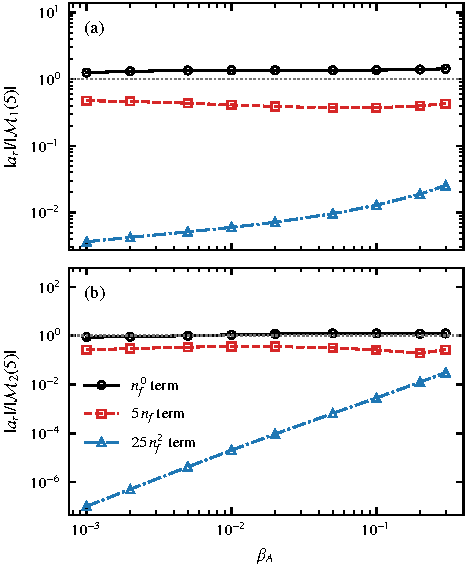
\includegraphics[width=\columnwidth]{figures/fig2_flavour.pdf}
 \caption{Magnitudes of the three terms of Eq.~\eqref{eq:nf5-sum}, divided by the magnitude of the complete coefficient, for $c=\BenchCos$, $\mA=\muR=\BenchMA\,\mathrm{GeV}$ and $\Nc=\BenchNc$. The horizontal line marks unity.}
 \label{fig:flavour-components}
\end{figure}

\begin{table}[t]
\centering
\caption{Evaluation time for the two complete Type II coefficients at the benchmark parameters, $c=\TimingCos$ and \TimingPrecision-digit working precision, for the unexpanded remainders (exact) and the series. First calls start with empty caches; repeated times are medians of \TimingRepeats{} evaluations at the same point. Starting the kernel and loading the files are excluded.}
\label{tab:timing}
\begin{ruledtabular}
\footnotesize
\setlength{\tabcolsep}{2.6pt}
\begin{tabular}{lcccccc}
& \multicolumn{3}{c}{first call [s]} & \multicolumn{3}{c}{repeated [s]} \\
$\bA$ & exact & series & ratio & exact & series & ratio \\
\hline
$1/10$ & 56.04 & 11.61 & 4.83 & 0.3422 & 0.0178 & 19.18 \\
$1/5$ & 45.68 & 11.64 & 3.92 & 0.3403 & 0.0179 & 18.99 \\
$3/10$ & 44.64 & 11.64 & 3.84 & 0.3485 & 0.0181 & 19.22 \\
\end{tabular}
\end{ruledtabular}
\end{table}



\emph{Scale dependence at two loops.} With the same ingredients, and with the subtraction operator $I^{(2)}$ of the original code, which, unlike Eq.~(3.4) of Ref.~\cite{Bhattacharya:2019bmd}, does not multiply the constant
\begin{align}
 H_g^{(2)}&=\tfrac12\Bigl[C_A^2\bigl(-\tfrac{5}{12}-\tfrac{11}{24}\zeta_2-\tfrac12\zeta_3\bigr)+C_A\nf\bigl(\tfrac{29}{27}+\tfrac{\zeta_2}{12}\bigr)
 \nonumber\\
 &\qquad-\tfrac12C_F\nf-\tfrac{5}{27}\nf^2\Bigr]
 \label{eq:H2}
\end{align}
by $(-\hat s/\muR^2)^{\epsilon}$, one finds
\begin{equation}
 \frac{\partial\Mfull{}}{\partial\ln\muR^2}=3\beta_0\,\mathcal M^{(1),\Fin}+\bigl(2\beta_1-8H_g^{(2)}-12C_F\nf\bigr)\mathcal M^{(0)},
 \label{eq:rg-two}
\end{equation}
where $\beta_1=\tfrac{34}{3}C_A^2-2C_F\nf-\tfrac{10}{3}C_A\nf$ and the last term comes from the counterterm of the $O_G$--$O_J$ amplitude, Eq.~\eqref{eq:gj-proportional}, in the renormalisation of Ref.~\cite{Bhattacharya:2019bmd}. We fitted $\partial\Mfull{}/\partial\ln\muR^2=a\,\beta_0\mathcal M^{(1),\Fin}+b\,\mathcal M^{(0)}$ to the series at two velocities and angles, for $(\Nc,\nf,\mA)=$ \RGSets. With both lines of Eq.~\eqref{eq:normalisation}, $a=\RGCoefficient$ to \RGaDev{} and $b$ agrees with Eq.~\eqref{eq:rg-two} to \RGbDev, the accuracy of the series at these velocities; the second derivative equals $6\beta_0^2\mathcal M^{(0)}$, the value implied by Eqs.~\eqref{eq:rg-one} and \eqref{eq:rg-two}, to \RGSecondDev. Without the division by \FileFactor{} the fit gives $a=\RGCoefficientPublished$, and without the scale term of the one-loop remainders $b$ differs from Eq.~\eqref{eq:rg-two} by $6\beta_0^2\ln(\mA^2/\mathrm{GeV}^2)$; the agreement therefore also fixes the reference scale of the published one-loop remainders at $\muR=1$~GeV.

\emph{Origin of the factor \FileFactor.} The Mathematica code of the original calculation documents it: the two-loop renormalisation step multiplies the $O_G$--$O_G$ amplitude, including the tree and one-loop amplitudes that enter the infrared subtraction, by $\FileFactor=\FileFactorRoot^2$, whereas the one-loop step does not. The pole cancellation of Ref.~\cite{Bhattacharya:2019bmd} is unaffected, since all terms of the two-loop subtraction carry the same factor. The released code and data use the normalisation of Eq.~\eqref{eq:normalisation}.

\emph{The original output.} The Mathematica output of the original calculation confirms both corrections. Its one-loop remainders, normalised to the tree amplitude, depend on $\muR$ as in Eq.~\eqref{eq:rg-one} and agree with the first line of Eq.~\eqref{eq:normalisation} to \ArchiveOneLoopDev; the published one-loop files coincide with them at $\muR=1$~GeV. An earlier version of the two-loop renormalisation step, without the factor \FileFactor{} and with the $O_J$ contribution switched off, was evaluated at $x=1/11$, $z=3/11$. At that point the published $P_1$ remainder equals \FileFactor{} times this result, multiplied by the tree amplitude, plus the $O_G$--$O_J$ counterterm of the published version; the real parts agree to \ArchiveTwoLoopDev. The imaginary parts differ by $32C_F$ times the one-loop $O_G$--$O_J$ amplitude, a multiple of the tree amplitude, so the two versions of the code treat this counterterm differently. In the normalisation of Eq.~\eqref{eq:normalisation} the difference is $24C_F\nf$ times the tree amplitude, which changes $\as^2V_2$ by \ArchiveOJShift; it belongs to the $O_J$ contribution discussed in Sec.~\ref{sec:rate}. The files and a script that reproduces these comparisons are part of the released material.

\section{Flavour decomposition}
\label{app:flavour}

% The timing table is defined here to control its placement.
\begin{table}[t]
\centering
\caption{Evaluation time for the two complete Type II coefficients at the benchmark parameters, $c=\TimingCos$ and \TimingPrecision-digit working precision, for the unexpanded remainders (exact) and the series. First calls start with empty caches; repeated times are medians of \TimingRepeats{} evaluations at the same point. Starting the kernel and loading the files are excluded.}
\label{tab:timing}
\begin{ruledtabular}
\footnotesize
\setlength{\tabcolsep}{2.6pt}
\begin{tabular}{lcccccc}
& \multicolumn{3}{c}{first call [s]} & \multicolumn{3}{c}{repeated [s]} \\
$\bA$ & exact & series & ratio & exact & series & ratio \\
\hline
$1/10$ & 56.04 & 11.61 & 4.83 & 0.3422 & 0.0178 & 19.18 \\
$1/5$ & 45.68 & 11.64 & 3.92 & 0.3403 & 0.0179 & 18.99 \\
$3/10$ & 44.64 & 11.64 & 3.84 & 0.3485 & 0.0181 & 19.22 \\
\end{tabular}
\end{ruledtabular}
\end{table}


To compare the sizes of the flavour contributions, I evaluate the decomposition of
Eq.~\eqref{eq:nf-decomposition} at $\nf=\BenchNf$:
\begin{align}
 \Mfull{i}(\BenchNf)
 &=\Mflav{i}{0}
   +\BenchNf\,\Mflav{i}{1}
   +\BenchNf^2\,\Mflav{i}{2}
 \nonumber\\
 &\equiv a_0+a_1+a_2,
 \qquad i=1,2.
 \label{eq:nf5-sum}
\end{align}
The index $i$ is suppressed in $a_r$. The factors $\BenchNf$ and $\BenchNf^2$
are included in $a_1$ and $a_2$, respectively, so these quantities are the three
terms entering the complete remainder, rather than the unweighted flavour coefficients.

Figure~\ref{fig:flavour-components} shows the magnitude of each term divided by
the magnitude of the complete remainder, $|a_r|/|\Mfull{i}(\BenchNf)|$, at
$c=\BenchCos$, $\mA=\muR=\BenchMA\,\mathrm{GeV}$ and $\Nc=\BenchNc$. Panels~(a) and~(b)
correspond to $\mathcal M_1$ and $\mathcal M_2$, respectively. Since the terms are
complex, their magnitudes do not add to the magnitude of their sum.
The plotted ratios therefore need not add to unity. A value above
the horizontal line at unity means that an individual term is larger
in magnitude than the complete remainder and is partly cancelled
by the other terms.

The term independent of $\nf$ is
the largest contribution to both coefficients over the plotted
range. The term linear in $\nf$ is also sizeable. For
$\mathcal M_1$, it partly cancels the $\nf^0$ contribution.
The overall cancellation among the three terms can be quantified
by
\[
 1-\frac{|a_0+a_1+a_2|}
          {|a_0|+|a_1|+|a_2|}.
\]
This quantity is zero when the terms add with the same phase
and increases as their sum is reduced by cancellation.
For $\mathcal M_1$, it lies between \PoneCancellationMin{}
and \PoneCancellationMax{} over the velocities shown.
These percentages refer to the reduction in magnitude relative
to $|a_0|+|a_1|+|a_2|$, not to a reduction in the cross section.

The relative signs of the flavour-dependent and gluonic
terms can also be seen in the leading power coefficients.
The combinations $\beta_0=(11\Nc-2\nf)/3$,
$\Nc a_{\mathrm A}-\nf a_{\mathrm F}$ and $4\Nc-\nf$ enter
$\widehat A_{12}$, $\widehat A_{11}$ and
$\widehat A_{21}$, respectively [Eqs.~\eqref{eq:leading-coefficients}
and \eqref{eq:M1-L1}]. They exhibit the relative minus
signs in the logarithmic terms; the size of the cancellation
in the complete remainder also depends on their phases and
on the powers of $\mathcal L$ that they multiply.

Finally, the $\nf^2$ contribution to $\mathcal M_2$ starts at
$\bA^2(1-c^2)$, as shown in Eq.~\eqref{eq:nf2-leading-two}.
This suppression explains why its relative contribution in
panel~(b) becomes small near threshold.

\section{Evaluation time and released data}
\label{app:data}

The series through $\bA^6$ occupy \SeriesKB~kB, against \PublishedTwoLoopMB~MB for the published two-loop files, a factor of \SizeRatio. The evaluation time was measured before the reduction of Sec.~\ref{sec:cancellations}, with the unexpanded expressions and the series in the forms used for the comparison of Sec.~\ref{sec:validation}, at $\bA=$ \TimingBetas, $c=\TimingCos$, $\mA=\muR=\TimingMA\,\mathrm{GeV}$ and $\Nc=\TimingNc$, with \TimingPrecision-digit working precision. On a first evaluation the series is \TimingFirstMin--\TimingFirstMax{} times faster. For repeated evaluations at the same point it is \TimingWarmMin--\TimingWarmMax{} times faster, with median \TimingWarmMedian; this does not correspond to a scan over new points. The two timed representations occupy \TimingSeriesMiB~MiB and \TimingExactMiB~MiB on disk, a factor of \TimingRepresentationRatio. Table~\ref{tab:timing} gives the individual measurements.
The measurements used Wolfram Language 13.2.0 for Linux x86 under Ubuntu 24.04.2 LTS on an AMD Ryzen 9 7950X processor with 124.9~GiB of memory.


The package contents and access details are given in Data Availability.
The construction files are organised by flavour coefficient and power of $\bA$, from $\bA^{-4}$ through $\bA^6$. The series are supplied in Wolfram Language form, with numerical evaluation code in Python and Wolfram Language.
The package contains \ValidationRows{} validation records and the forward angle data.
The construction and validation code is written in Wolfram Language, C++ and Python.
The construction files and validation records are checked against the outputs of the original runs, and a script repeats the construction from the published expressions.
Each table, figure and number in this paper is generated from these data by a single command, including the check of the DPS weight in Fig.~\ref{fig:dps}, the logarithms of Sec.~\ref{sec:rate} and the normalisation checks of App.~\ref{app:normalization}.
A test suite checks the numerical evaluation code against the validation records.
Only the construction of the series from the unexpanded expressions requires Mathematica.
The series are intended for $\bA\leq\RecommendedBeta$ at the angles tested (Sec.~\ref{sec:use}).
Outside this range, use the unexpanded remainders.


% Page markers for scripts/check_layout.py (no output).
\label{end-of-appendices}
%\FloatBarrier
\label{start-of-references}
\bibliography{references}

\end{document}
